%                                                                 aa.dem
% AA vers. 8.2, LaTeX class for Astronomy & Astrophysics
% demonstration file
%                                                       (c) EDP Sciences
%-----------------------------------------------------------------------
%
%\documentclass[referee]{aa} % for a referee version
%\documentclass[onecolumn]{aa} % for a paper on 1 column  
%\documentclass[longauth]{aa} % for the long lists of affiliations 
%\documentclass[rnote]{aa} % for the research notes
%\documentclass[letter]{aa} % for the letters 
%\documentclass[bibyear]{aa} % if the references are not structured 
% according to the author-year natbib style

%
\documentclass{aa}  
\usepackage{caption}
\usepackage{graphicx,subcaption}
%%%%%%%%%%%%%%%%%%%%%%%%%%%%%%%%%%%%%%%%
\usepackage{txfonts}

%%%%%%%%%%%%%%%%%%%%%%%%%%%%%%%%%%%%%%%%
%\usepackage[options]{hyperref}
% To add links in your PDF file, use the package "hyperref"
% with options according to your LaTeX or PDFLaTeX drivers.
%
\begin{document} 


   \title{Spectroscopic Analysis of Fornax Dwarf Galaxies}

   \subtitle{I. Kinematics \& Kinematic Scaling Relation}

   \author{F. S. Eftekhari\inst{1,2}, R. Peletier\inst{1},  N. Scott\inst{3}, \and S. Mieske\inst{2}}

   \institute{Kapteyn Astronomical Institute, Postbus 800, 9700 AV Groningen, The Netherlands         \and
             European Southern Observatory, Alonso de C$\acute{o}$rdova 3107, Vitacura, Santiago, Chile    
         \and
             ??}

   \date{Received October 1, 2019; accepted March 15, 2020}

% \abstract{}{}{}{}{} 
% 5 {} token are mandatory
 
  \abstract
  % context heading (optional)
  % {} leave it empty if necessary  
   {\bigskip}
  % aims heading (mandatory)
   {\bigskip}
  % methods heading (mandatory)
   {\bigskip}
  % results heading (mandatory)
   {\bigskip}
  % conclusions heading (optional), leave it empty if necessary 
   {}

   \keywords{\bigskip}

   \maketitle
%
%________________________________________________________________

\section{Introduction}

%\begin{itemize}
%	\item (DONE) Evolution of galaxies in clusters and environmental effects, finishing with explaining harassment \& ram-pressure stripping
%	\item (DONE)These effects in Fornax cluster(why Fornax), finishing with details of Fornax 
%	\item (DONE) Dwarf are more vulnerable to environment, what dwarfs are, and what are the discoveries about dwarfs
%	\item SAMI (how we approach these problems) \& FDS catalog
%	\item sections of this paper
%\end{itemize}

% Dwarfs (1) what they are (2) what we know till now about them (2) why studying is important (4) open questions
%Talk about Fornax cluster, (1)it's environment, (2) the previous studies done on it, (3) why studying it is important (4) why now and how can we do it
% FDS (1) what is it (2) how we are using it
% SAMI What is it and why we chose it

   Still after decades of studying dwarf galaxies, the formation and evolution of these objects is considered an active debate. Over the past few years, alongside improvement of observation the idea behind the lifeline of these faint and small objects had become clearer (e.g. Ry$\acute{s}$ et al. 2013, Toloba et al. 2015, Venhola et al. 2018). However, the need for more detailed and precise data to close this debate is still on the table. Thus with high resolution multiplexing deep-SAMI data cubes and statistically significant sample of dEs in Fornax cluster, we've started a new journey to collect new information from kinematics, chemical composition and structure of these faint objects. Why studying these faint objects is important, how we approached these questions, and what new results and clues are accomplished are the questions which are going to be investigated in this research.

%\subsection{Why Fornax cluster? Why dwarf galaxies?}
Different theories and ideas about the formation history and evolution of the big zoo of galaxies in different environments have been developed in the past decades. Dressler (1980) discovered the commonness of each galaxy morphology in different environment, as which in the local Universe red early-type galaxies mostly appear in dense regions while late-type spiral galaxies tend to avoid higher density environments. Notably low mass galaxies such as dwarf elliptical galaxies are seen as the dominant population in  in big groups and clusters (Binggeli et al. 1990, Moore et al. 1998, Boselli et al. 2008; Serra et al. 2012 etc.). Luminosity function of galaxies within cluster and field are also seen to be strongly different (Binggeli et al. 1988). The strong morphology-density relation in nearby galaxy clusters (Cappellari 2016) indicates that for galaxies inside clusters one of the main drivers of their evolution is environmental effect such as ram-pressure stripping (Lin \& Faber 1983), harassment (Moore et al. 1998), or starvation (Larson et al. 1980). 
Galaxies upon accretion into the dense environment of galactic clusters and while passing through the intracluster medium with high velocity experience various environmental mechanisms. In clusters with large mass ($\sim10^{14-15}M_{\odot}$) and so strong potential well repeated tidal interactions occur between high velocity galaxies and between galaxies and the cluster potential. This effect which is called harassment influences stellar mass, dark matter and gas content of the galaxy and can convert morphology of the object (Mastropeitro et al. 2005, Fujita 1998). As the outskirt of the galaxy is ripped off galaxies become more compact and their size will be changed (Janze et al. 2016a), but the strength of mass loss from harassment is quite dependent on the orbital velocity of the galaxy (Mastropietro et al. 2005; Smith et al. 2010, 2013 and 2015). Another environmental process is ram-pressure stripping. The deep cluster gravitational potential derives high orbital velocities and hot ionized gas. In clusters with hot gas especially nearby their centers, cold gas component of the galaxy will be partly removed in each crossing through the hot emitting gas of the cluster (Gunn \& Gott 1972, ). Dwarf galaxies with blue center (Lisker et al. 2006), HI tails of in-falling late-type galaxies (Kenney et al. 2004; Jaffe et al. 2018) and the gas richness of field galaxies compared to cluster galaxies (Solanes et al. 2001; Serra et al. 2012) are indications of ram-pressure in clusters. When ram-pressure stripping is strong it can remove the atomic gas disk (Boselli et al. 2008) and when it's not strong enough it can still strip away the warm ionized halo gas of the galaxy (Font et al. 2008; McCrthy et al. 2008; Bekki 2009). This process is known as starvation and stops the cooling process of hot halo and so forcing the galaxy to use up its last disk gas (Larson et al. 1980).

Fornax cluster with the distance of 19.95 Mpc (Tonry et al. 2001) and the distance modulus of 31.43 is the second closest cluster to us. Compared to Virgo cluster it's older and more dynamically evolved, but less studied. It's smaller, denser and has still very active environment (Zabel et al. 2019) that strongly influences even the tightly bound molecular gas of its members. This cluster with the central mean recession velocity of $1493\pm36$ $km^{-1}$, a virial mass of $M=7\times10^{13}M_{\odot}$ and virial radius of $4^{\circ}$ or 1.4 Mpc is located in the southern sky in the Fornax-filament of the cosmic web (Nasonova et al. 2011) and consist of hundreds of faint galaxies $M_B>-18$ (Ferguson 1989; Venhola et al. 2018). Fornax cluster despite its low mass has very dense center similar to central density of the more massive Virgo cluster, and so galaxies in the cluster core tend to experience frequent tidal interactions with other galaxies, their material be ripped off and become denser, harassment. Moreover the intensity of the hot X-ray gas in the inner cluster $100$ kpc (Paolilloet al. 2002) with a mass of $M\approx 10^{11}M_{\odot}$ increases the chances of ram pressure stripping and so changing stellar population of its galaxies. The dynamically evolved center of the cluster and evolved galaxy population are a signature that galaxies have spent few Gyrs in the cluster environment and travelled few times through the cluster center (Drinkwater et al. 2001) and consequential significant intracluster stars (Pota et al. 2018). Specially dwarf galaxies through strong gravitational interactions can end up completely disrupted and filling up the intracluster medium (McGlynn 1990; Koch et al. 2012). Also the high fraction of early-type galaxies $87\%$ (Ferguson 1989) suggest that during their stay in the cluster they were not forming many stars.

%\subsection{What do we know about dwarfs?}
Faint objects such as dwarf galaxies because of their low mass and so lower gravitational potential are powerful probes to environmental processes. Dwarf galaxies despite their plain appearance and smooth light distribution have complex characteristics (Lisker 2006), which indicate the influence of environment in their past. \textit{Spatial distribution of dwarfs}: early-type dwarf galaxies (dEs) outnumber all other galaxy types in dense environment, like clusters, while late-type low-luminosity galaxies are the dominant population in the fields (e.g. Dressler 1980, Sandage et al. 1985, and Ferguson \& Bingelli 1994). \textit{Inner structure vs. local density of dEs}: A substructure-density relation is seen in early-type dwarf galaxies, such that dEs with blue center or no nucleus are mostly found in low-density cluster regions, dEs with disks in intermediate-density regions, and nucleated dEs in high-density regions of the cluster (Ferguson \& Sandage 1989, van den Bergh 1986, and Lisker et al. 2007). \textit{Color vs. local density of dEs}: dEs in higher density regions are redder compared to other regions (Lisker et al. 2008). \textit{Kinematics vs. local density of dEs}: pressure supported dEs are mostly found in high density regions of cluster, whereas in lower density regions like outskirts the angular momentum of dEs increases and dEs are largely rotationally supported. Also fast rotators in the outer part of the cluster rotate faster than fast rotators in the inner parts of the cluster (Toloba et al. 2009, van Zee et al. 2004a, and Toloba et al. 2015). Dwarf galaxies's formation history is another key to the formation and evolution of galaxies; whether dwarf galaxies are the descendants in hierarchical structure formation (Moore et al. 1999) and were created by gravitational collapse like other galaxies (Kauffmann \& White 1993), or whether they were formed at later epoch from late-type low-luminosity star forming galaxies by environmental effects (Boselli \& Gavazzi 2006, Gavazzi et al. 2013, and Boselli \& Favazzi 2014). The answer to these questions could be achieved by pursuing the behaviour and location of these galaxies inside galaxy physical parameter space. \textit{Surface brightness profile}: logarithm of the S$\acute{e}$rsic index of both dwarfs and giant early-type galaxies linearly increases with central surface brightness and magnitude, but SB profiles of dEs are less steep than massive ellipticals (Gavazzi et al. 2005, Graham \& Guzm$\acute{a}$n 2013, and Young \& Currie 1994). \textit{Color magnitude relation}: there is no gap seen between dwarfs and giant ellipticals in color magnitude profile (e.g. Ferrarese et al. 2006, Janz \& Lisker 2009, and Misgeld et al. 2008\&2009). \textit{Fundamental plane}: inside fundamental plane it's been seen that dEs are offset with respect to the plane of early-type galaxies (Toloba et al. 2012 and Rijcke et al. 2015). \textit{Disky substructure}: disk-like structures have been seen in fast rotators and dEs in the outer regions of cluster, also they have rotation curves similar to those of late-type galagixes (Toloba et al. 2015 and Toloba et al. 2009). \textit{Star formation}: As the galay's luminosity decreases the duration of star formation increases (Gavazzi et al. 2002), also $H_\beta$ absorption index increases from giants to dwarfs as luminosity and velocity dispersion decreases (Poggianti et al. 2001 and Geha et al 2003). 

 This is the second paper of the SAMI Fornax Dwarfs Survey series, and is dedicated to kinematic studies of dwarf early-type galaxies within Fronax galaxy cluster. In sect. 2 we describe the SAMI Fornax IFU data set, its comparison to previous observations, and the chosen photometric catalog. The methods used for an section 3 \& 4, we'll explain the methods that have been used and our results respectively. Finally, Section 5 will present the discussion and conclusions.   





%__________________________________________________________________
\section{Data}

\begin{table}
\centering
\caption{Projects on Dwarf Galaxies} % title of Table
\resizebox{\columnwidth}{!}{%
\begin{tabular}{cccccc} % centered columns (4 columns)
\hline\hline\\ %inserts double horizontal lines
Survey & No. & $\lambda$ & FWHM & Cluster & Telescope \\ [0.5ex] % inserts table
\hline\\
&& 4660-5430 (B)& 1.0\\[-1ex]
\raisebox{1.5ex}{SAMI\_Fornax} &\raisebox{1.5ex}{60}& 6250-7350 (R) &1.6 &  \raisebox{1.5ex}{Fornax} & \raisebox{1.5ex}{SAMI@AAO} \\ [1ex]
\hline\\
SAURON &12& 4760-5300 & 3.9 & Virgo & WHT@ING \\
\hline\\ % inserts single horizontal line
 &10& 4600-5600 & 1.6 & Virgo & INT@ING\\ % inserting body of the table
&&4200-5000 (B) &1.4 \\[-1ex]
\raisebox{1.5ex}{SMACKED}&\raisebox{1.5ex}{26} &5500-6700 (R)& 3.2 & \raisebox{1.5ex}{Virgo} & \raisebox{1.5ex}{WHT@ING} \\
 &3& 4500-5600 & 2.7 & Virgo &  VLT@ESO\\
\hline\\\
&& 3500-7100 (B)& 1.6 & &WHT\&INT@ING\\[-1ex]
\raisebox{1.5ex}{MAGPOP} &\raisebox{1.5ex}{4}& 8000-9100 (R) &3.2 &  \raisebox{1.5ex}{Virgo} & TNG@INAF \\ [1ex] % [1ex] adds vertical space

\hline
\end{tabular}
}
\label{CompDwrf} % is used to refer this table in the text
\end{table}

\begin{table*}
\begin{center}
\caption{}
{\renewcommand{\arraystretch}{1.}
\resizebox{18cm}{!} {
\begin{tabular}{|ccccccccccc|}
\hline 
FCC name & FDS name & year & RA & DEC & $R_e$ & $M_r$ & $\mu_r$  & $\epsilon$ & n & g-r \\ 
 &  &  & (deg) & (deg) & (arcsec) & (mag) & ($mag/arcsec^2$) &  & & (mag)\\
\hline \hline
FCC213 & FDS11\_DWARF003 & 2016 & 54.620899 & -35.450439 & 114.88$\pm$8.41 & -23.02$\pm$0.08 & 20.70$\pm$0.23 & 0.92 & 5.80 & 0.84\\
FCC167 & FDS11\_DWARF006 & 2016 & 54.115009 & -34.976017 & 44.49$\pm$2.49 & -22.01$\pm$0.06 & 19.18$\pm$0.17 & 0.59 & 2.88 & 0.73\\
FCC219 & FDS11\_DWARF166 & 2016 & 54.716400 & -35.593323 & 26.15$\pm$1.09 & -22.00$\pm$0.05 & 18.45$\pm$0.13 & 0.87 & 3.60 & 0.82\\
FCC184 & FDS11\_DWARF001 & 2016 & 54.237602 & -35.506592 & 73.56$\pm$5.68 & -21.84$\pm$0.09 & 20.91$\pm$0.24 & 0.93 & 7.47 & 0.87\\
FCC276 & FDS6\_DWARF001 & 2018 & 55.580955 & -35.392532 & 110.84$\pm$11.36 & -21.62$\pm$0.11 & 21.72$\pm$0.32 & 0.70 & 7.85 & 0.73\\
FCC29 & FDS25\_DWARF000 & 2018 & 50.984844 & -36.464443 & 43.82$\pm$2.72 & -21.56$\pm$0.07 & 19.92$\pm$0.19 & 0.81 & 5.43 & 0.76\\
FCC179 & FDS12\_DWARF003 & 2016 & 54.192539 & -35.999268 & 74.62$\pm$6.79 & -21.23$\pm$0.10 & 20.84$\pm$0.29 & 0.48 & 6.86 & 0.73\\
FCC147 & FDS16\_DWARF001 & 2016 & 53.819111 & -35.226257 & 29.51$\pm$1.67 & -21.08$\pm$0.06 & 19.75$\pm$0.17 & 0.98 & 5.39 & 0.75\\
FCC83 & FDS19\_DWARF000 & 2018 & 52.645653 & -34.853939 & 55.35$\pm$4.74 & -20.82$\pm$0.10 & 20.87$\pm$0.27 & 0.61 & 6.81 & 0.80\\
FCC193 & FDS11\_DWARF000 & 2016 & 54.298901 & -35.746105 & 15.53$\pm$0.74 & -20.34$\pm$0.05 & 18.67$\pm$0.15 & 0.66 & 3.09 & 0.75\\
FCC153 & FDS15\_DWARF002 & 2016 & 53.87944 & -34.447021 & 23.15$\pm$1.66 & -19.62$\pm$0.08 & 18.63$\pm$0.22 & 0.15 & 1.62 & 0.74\\
FCC177 & FDS10\_DWARF000 & 2016 & 54.197838 & -34.739735 & 28.81$\pm$2.51 & -19.34$\pm$0.10 & 20.01$\pm$0.27 & 0.26 & 1.66 & 0.69\\
FCC249 & FDS13\_DWARF000 & 2018 & 55.175434 & -37.510769 & 7.13$\pm$0.30 & -19.21$\pm$0.05 & 18.54$\pm$0.12 & 0.98 & 3.47 & 0.81\\
FCC190 & FDS11\_DWARF005 & 2016 & 54.287319 & -35.195053 & 16.23$\pm$1.07 & -19.19$\pm$0.07 & 20.28$\pm$0.20 & 0.92 & 1.81 & 0.85\\
\hline
FCC277 & FDS6\_DWARF002 & 2018 & 55.594924 & -35.154098 & 11.44$\pm$0.68 & -18.82$\pm$0.07 & 19.39$\pm$0.18 & 0.58 & 1.89 & 0.65\\
FCC143 & FDS16\_DWARF002 & 2016 & 53.746666 & -35.171089 & 9.81$\pm$0.56 & -18.66$\pm$0.06 & 19.63$\pm$0.17 & 0.85 & 4.34 & 0.74\\
FCC235 & FDS11\_DWARF519 & 2016 & 55.041069 & -35.629093 & 42.30$\pm$5.54 & -18.57$\pm$0.14 & 22.64$\pm$0.42 & 0.68 & 0.85 & 0.34\\
FCC301 & FDS7\_DWARF000 & 2018 & 56.264900 & -35.972668 & 7.60$\pm$0.41 & -18.34$\pm$0.06 & 18.89$\pm$0.16 & 0.54 & 2.12 & 0.72\\
FCC263 & FDS5\_DWARF000 & 2018 & 55.385574 & -34.888752 & 16.47$\pm$1.38 & -18.28$\pm$0.09 & 20.51$\pm$0.26 & 0.48 & 1.37 & 0.48\\
FCC37 & FDS25\_DWARF241 & 2018 & 51.289337 & -36.365185 & 33.89$\pm$4.35 & -18.17$\pm$0.14 & 22.56$\pm$0.41 & 0.68 & 1.09 & 0.45\\
FCC33 & FDS26\_DWARF003 & 2018 & 51.243237 & -37.009613 & 16.89$\pm$1.51 & -18.07$\pm$0.10 & 20.50$\pm$0.28 & 0.37 & 1.18 & 0.66\\
FCC285 & FDS7\_DWARF360 & 2018 & 55.760147 & -36.273357 & 32.65$\pm$4.32 & -17.97$\pm$0.15 & 22.78$\pm$0.42 & 0.74 & 1.22 & 0.37\\
FCC182 & FDS11\_DWARF279 & 2016 & 54.226295 & -35.374714 & 9.67$\pm$0.66 & -17.89$\pm$0.08 & 20.50$\pm$0.21 & 0.96 & 2.43 & 0.81\\
FCC136 & FDS16\_DWARF159 & 2016 & 53.622837 & -35.546459 & 17.50$\pm$1.72 & -17.77$\pm$0.11 & 21.78$\pm$0.31 & 0.85 & 2.14 & 0.78\\
FCC106 & FDS15\_DWARF417 & 2018 & 53.198673 & -34.238728 & 10.65$\pm$0.87 & -17.42$\pm$0.09 & 20.44$\pm$0.26 & 0.49 & 2.18 & 0.68\\
FCC202 & FDS11\_DWARF235 & 2015 & 54.527325 & -35.439911 & 13.28$\pm$1.25 & -17.34$\pm$0.11 & 21.21$\pm$0.30 & 0.59 & 1.67 & 0.73\\
FCC113 & FDS15\_DWARF107 & 2018 & 53.279419 & -34.805576 & 18.92$\pm$2.35 & -17.04$\pm$0.14 & 22.45$\pm$0.39 & 0.69 & 1.19 & 0.48\\
FCC222 & FDS11\_DWARF283 & 2015 & 54.805500 & -35.371410 & 16.10$\pm$1.86 & -16.97$\pm$0.13 & 22.44$\pm$0.36 & 0.89 & 1.35 & 0.69\\
FCC100 & FDS16\_DWARF417 & 2018 & 52.948479 & -35.051388 & 19.77$\pm$2.56 & -16.96$\pm$0.14 & 22.72$\pm$0.41 & 0.76 & 1.46 & 0.71\\
FCC203 & FDS10\_DWARF189 & 2016 & 54.538200 & -34.518761 & 16.04$\pm$1.88 & -16.90$\pm$0.13 & 21.97$\pm$0.37 & 0.55 & 1.46 & 0.66\\
FCC135 & FDS15\_DWARF384 & 2016 & 53.628445 & -34.297371 & 14.72$\pm$1.68 & -16.82$\pm$0.13 & 21.70$\pm$0.36 & 0.47 & 1.58 & 0.64\\
FCC207 & FDS11\_DWARF396 & 2015 & 54.580185 & -35.129124 & 9.59$\pm$0.92 & -16.59$\pm$0.11 & 21.63$\pm$0.30 & 0.83 & 1.54 & 0.66\\
FCC245 & FDS11\_DWARF458 & 2018 & 55.140991 & -35.022888 & 14.52$\pm$1.78 & -16.50$\pm$0.14 & 22.72$\pm$0.39 & 0.92 & 1.51 & 0.62\\
FCC252 & FDS11\_DWARF069 & 2018 & 55.209988 & -35.748455 & 11.13$\pm$1.21 & -16.41$\pm$0.12 & 22.25$\pm$0.34 & 0.94 & 1.21 & 0.69\\
FCC300 & FDS7\_DWARF326 & 2018 & 56.249588 & -36.319752 & 20.82$\pm$3.23 & -16.38$\pm$0.17 & 23.37$\pm$0.49 & 0.72 & 1.14 & 0.67\\
FCC266 & FDS6\_DWARF455 & 2018 & 55.422161 & -35.170265 & 6.91$\pm$0.58 & -16.35$\pm$0.09 & 21.23$\pm$0.26 & 0.89 & 1.17 & 0.66\\
FCC46 & FDS22\_DWARF244 & 2018 & 51.604301 & -37.127785 & 8.51$\pm$0.82 & -16.31$\pm$0.11 & 21.35$\pm$0.30 & 0.64 & 0.98 & 0.49\\
FCC188 & FDS11\_DWARF155 & 2015 & 54.268906 & -35.590149 & 12.20$\pm$1.45 & -16.26$\pm$0.13 & 22.64$\pm$0.38 & 0.96 & 1.00 & 0.69\\
FCC211 & FDS11\_DWARF339 & 2015 & 54.589504 & -35.259689 & 6.58$\pm$0.58 & -16.11$\pm$0.10 & 21.17$\pm$0.27 & 0.75 & 1.66 & 0.64\\
FCC164 & FDS12\_DWARF367 & 2016 & 54.053589 & -36.166451 & 9.95$\pm$1.13 & -16.00$\pm$0.13 & 21.85$\pm$0.36 & 0.55 & 1.47 & 0.63\\
FCC306 & FDS7\_DWARF310 & 2018 & 56.439095 & -36.346100 & 7.26$\pm$0.71 & -15.91$\pm$0.11 & 21.33$\pm$0.31 & 0.59 & 0.90 & 0.32\\
FCC253 & FDS13\_DWARF042 & 2018 & 55.230301 & -37.837627 & 10.92$\pm$1.36 & -15.83$\pm$0.14 & 22.35$\pm$0.39 & 0.62 & 1.13 & 0.71\\
FCC274 & FDS6\_DWARF208 & 2015 & 55.571922 & -35.540737 & 12.05$\pm$1.62 & -15.75$\pm$0.15 & 23.12$\pm$0.43 & 0.96 & 1.26 & 0.58\\
FCC298 & FDS6\_DWARF098 & 2018 & 56.185070 & -35.683716 & 6.97$\pm$0.71 & -15.62$\pm$0.11 & 21.73$\pm$0.32 & 0.71 & 1.19 & 0.62\\
FCC264 & FDS6\_DWARF170 & 2015 & 55.382313 & -35.589550 & 10.27$\pm$1.34 & -15.51$\pm$0.14 & 22.06$\pm$0.41 & 0.40 & 1.05 & 0.58\\
FCC195 & FDS10\_DWARF014 & 2016 & 54.347183 & -34.900108 & 12.78$\pm$1.92 & -15.44$\pm$0.16 & 22.92$\pm$0.48 & 0.54 & 1.06 & 0.66\\
FCC250 & FDS13\_DWARF258 & 2018 & 55.184971 & -37.408268 & 9.22$\pm$1.27 & -15.06$\pm$0.15 & 22.97$\pm$0.44 & 0.76 & 0.84 & 0.72\\
FCC178 & FDS10\_DWARF302 & 2016 & 54.202728 & -34.280102 & 11.26$\pm$1.76 & -15.02$\pm$0.17 & 23.37$\pm$0.50 & 0.71 & 1.24 & 0.58\\
FCC134 & FDS15\_DWARF223 & 2016 & 53.590393 & -34.592522 & 6.52$\pm$0.84 & -14.60$\pm$0.14 & 22.36$\pm$0.41 & 0.57 & 0.81 & 0.48\\
FCC51 & FDS21\_DWARF129 & 2018 & 51.776043 & -36.636787 & 4.45$\pm$0.52 & -14.15$\pm$0.13 & 22.21$\pm$0.37 & 0.70 & 0.96 & 0.64\\ 
\hline
\end{tabular}
}}
\end{center}
\end{table*}

The SAMI Fornax project started in 2015 with the Sydney-AAO Multi-Object Integral-field (SAMI) spectrograph on the Anglo-Australian Telescope (AAT), with aim of studying the origin and the inner workings of dwarf galaxies inside Fornax cluster. As results of total 17 allocated nights in 2015B, 2016B and 2018B, we have 38 dwarf galaxies ($M_r>-19$), 12 giant elliptical galaxies with successful stellar kinematic measurements. The observing strategy and in detail description of the sample is described in paper I by N. Scott et al. (2019), but for completeness a short description will also be given here. 

SAMI is an integral-field spectrograph equipped by 13 fiber-based IFUs called hexabundles, and 26 pluggable sky fibers (Bryant et al. 2014). Each hexabundle with a field-of-view of $15''$ diameter, is made of 61 1.6-arcsecond optical fibers. These hexabundles have physical size <1 mm, with a filling fraction of 73 per cent and together with sky fibers each fits into pre-drilled holes in a field plate. The plug plate with about 1 degree field-of-view is installed a the AAT's Prime Focus Camera top end and so hexabundle's face is placed at the focal plane of the telescope. 
To study structure of low-mass galaxies such as dEs in Fornax cluster, high resolution spectra and high S/N were needed. With 
the  double-armed AAOmega spectrograph having 1500V gratings in blue and 100R gratings in red, our data has resolution of ~5100 (FWHM $= 1.0 \AA$) in blue ($\sim4660-5430\AA$) and ~4300 (FWHM $= 1.6 \AA$) in red ($6250-7350A^o$). Which means successfully reaching around 12 km/s and 15 km/s velocity dispersions in blue and red respectively. And with fourteen ~30 minutes exposure times for each field gaining high S/N became possible. \\
Compared to single IFU instruments SAMI could simultaneously observe 12 galaxies and one calibration star which significantly increases the observation rate.
Also most of the previous surveys are long slit, which make them susceptible to aperture effects, while Integral Field Spectroscopy spatially resolves each galaxy and gives different spectra at different parts of the galaxy. Current IFU surveys (e.g. SAMI Galaxy Survey, MANGA) are not useful for the study of dEs due to sensitivity, effective spatial resolution and most importantly spectral resolution limitations. A comparison between theses projects can be seen in table 1.

Our science targets were selected in 2015 from Fornax Cluster Catalog (FCC, Feguson 1989) and in 2016 \& 2018 from Fornax Deep Survey (FDS, Venhola et al. 2018) dwarf galaxy catalog. Since the aim was to study star formation and evolution of dwarf-elliptical galaxies within Fornax cluster, the primary survey targets are dEs that cover $ -18<M_r<-14.5$ and $17<\mu_r<23$, however to allocate all 13 hexabundles of each pointing of the $1^o$ diameter plate other dwarf galaxies, giant ellipticals even background galaxies were also included in the target selection. 
The observations covered 90 objects in the main cluster up to $2^o$  away from the NGC 1399, and 9 objects in Fornax A, even though about half of them were excluded since their spectra were too faint and noisy to measure their kinematic parameters. In detail description of the methods used for analysis of IFU spectra will be followed in the next section. 

The sample selection was mainly done by deep imaging data from the Fornax Deep Survey (Venhola et al. 2018) dwarf galaxy catalog. This multiband optical images ($\approx1$ arcsec) include 564 dwarf galaxies in the Fornax cluster and the in-falling Fornax A subgroup. The survey was excecuted using the OmegaCAM (Kuijken et al. 2002) instrument on the survey telescope of the 2.6m Very Large Telescope (Schipani et al. 2012) in Cerro Paranal, Chile. FDS cover a 26 deg$^2$ area of the cluster up to its virial radius in u$'$, g$'$, r$'$, and i$'$ bands, with the liming magnitude of $M_{r'}=-10.5$ mag, and the limiting mean effective surface brightness of  $\bar{\mu}_{e,r'}=26$ mag arcsec$^{-2}$. The detail of 50 SAMI Fornax galaxies are presented in table 4. For further photometric parameters refer to FDS catalog. 


\section{Methods}
To extract stellar kinematics or stellar population (Paper III) from absorption-line spectra of galaxies we used the Penalized Pixel-Fitting (pPXF) routine of Cappellari \& Emsellen (2004). pPXF basically is a maximum penalized likelihood approach in pixel space, with the aim of finding an optimal template with the minimum template-galaxy mismatch errors. It finds the best-fitting linear combination of input stellar templates by convolving them with the line-of-sight velocity distribution of the input galaxy's spectra, and then the best-fitting parameters are determined by non-linear chi-squared minimization in pixel space (logarithmically binned in wavelength). During fitting we are extracting the first four Gauss-Hermite moments of the LOSVD (V, $\sigma$, $h_3$, and $h_4$) as far as the S/N of the galaxies accompany.
For the optimized fitting we include an additive Legendre polynomial of 6th degree and a multiplicative Legendre polynomial of 10 order to correct the stellar template continuum shape. The additive polynomials minimize template mismatch and additionally correct for imperfect sky subtraction. The multiplicative polynomials  correct for imprecision in primary calibration of the spectra and make the fit insensitive to reddening by dust. The best match to SAMI-Fornax's wavelength range and spectral resolution is the empirical single-age single-metallicity population template library Pegase-HR (Le Borgne et al. 2004). Pegase-HR is based on ELODIE, which is a high resolution stellar library of 1959 spectra for 1503 stars with R$=10000$ at $\lambda=550$ nm. The spectra of some of SAMI-Fornax galaxies and their corresponding fits are shown for the blue range in Fig. 1. The black spectrum shows the galaxy spectrum, and the overplotted purple spectrum is the best-fitting stellar template. Below each spectrum, the differences between the galaxy spectrum and the best stellar template are shown as green dots which have beed arbitrarily shifted in the vertical direction for better presentation. \textbf{[add some spectra fitting examples]}\\
To get a reliable measurement of stellar kinematics a minimum S/N must be available. In our case a $(S/N)_{min}=10$ for velocity and $(S/N)_{min}=15$ for velocity dispersion profiles were efficient. This is achievable by adaptive voronoi binning method of Cappellari \& Copin (2003) in which starting from central pixel the spectra of the neighbouring pixels will be added till the the target S/N is reached. As result the size of bins become larger as they get to outskirts of the galaxies. Then to get a radial profile of each parameter pPXF was run on each Voronoi-binned spectrum. \textbf{[add a map of Fornax cluster in data section and few smaples of maps in the map then refer to them here]}
In the sample, some galaxies were found to exhibit emission lines, which in these cases we're allowing emission-line regions to be easily masked. Galaxies with prominent emission lines are FCC179, FCC184, FCC29, FCC33, FCC263, FCC181. 
Errors were estimated through Monte Carlo simulation, in which the input spectrum is perturbed by random values convolved by the sigma of the difference between original and best-fitted template spectra. After around 100 realization, the mean and sigma of the distribution of each kinematic parameter will be calculated, and this sigmas are estimates of the errors.

%N. Kacharov et al. 2018 --> The SSP models are computed using the Padova isochrones (Bertelli et al.1994), assuming a Kroupa initial mass function (IMF; Kroupa 2001), and normalized to present day mass of 1 Solar mass. They include mass loss from supernovae ejecta (Woosley  &  Weaver 1995)  and  stellar  winds.  They  have  a  resolution R=10^4 and  cover  a  wavelength  range  between  3900 and 6800 �. The grid covers seven metallicity bins with a range −2.3<[Fe/H]<+0.7, assuming a scaled Solar abundance pattern, and 68 irregularly spaced age bins between 1 Myr and 20 Gyr.

%In pPXF one can also fit the gas emission lines together with the stellar kinematics and population. But for the current work since not all of the galaxies have emission lines, we avoid regions with emission lines by simply masking them to gain the best fitting spectra. 

%Another interesting feature in this method is regularization which is used to reduce the noise in the recovery of the stellar population parameters and more importantly it attaches a physical meaning to the output weights assigned to the best-fitting template in term of the star formation history (SFH) or metallicity distribution of each galaxy. This feature was important in stellar population of our galaxies (SAMI-Fornax paper 3).

%In order to check the accuracy of our results, we compared them with Toloba et al. 2011 study on dwarf galaxies which can be seen in plot ??. Our measurement show ...

\section{Scaling Relations}
To understand the origin of dwarf galaxies, the role of environment in evolution of these low-mass stellar systems and also their dark matter content, we analyze their scaling relations and how deviations from them depend on kinematics or stellar population of galaxies. Manifolds of galaxy properties such as the Faber-Jackson, the fundamental Plane (FP), the color-velocity dispersion relation, and etc. \textbf{[Say more about scaling relations in general]}

\section{Faber Jackson}

\begin{figure*}[!htb]
   \centering
	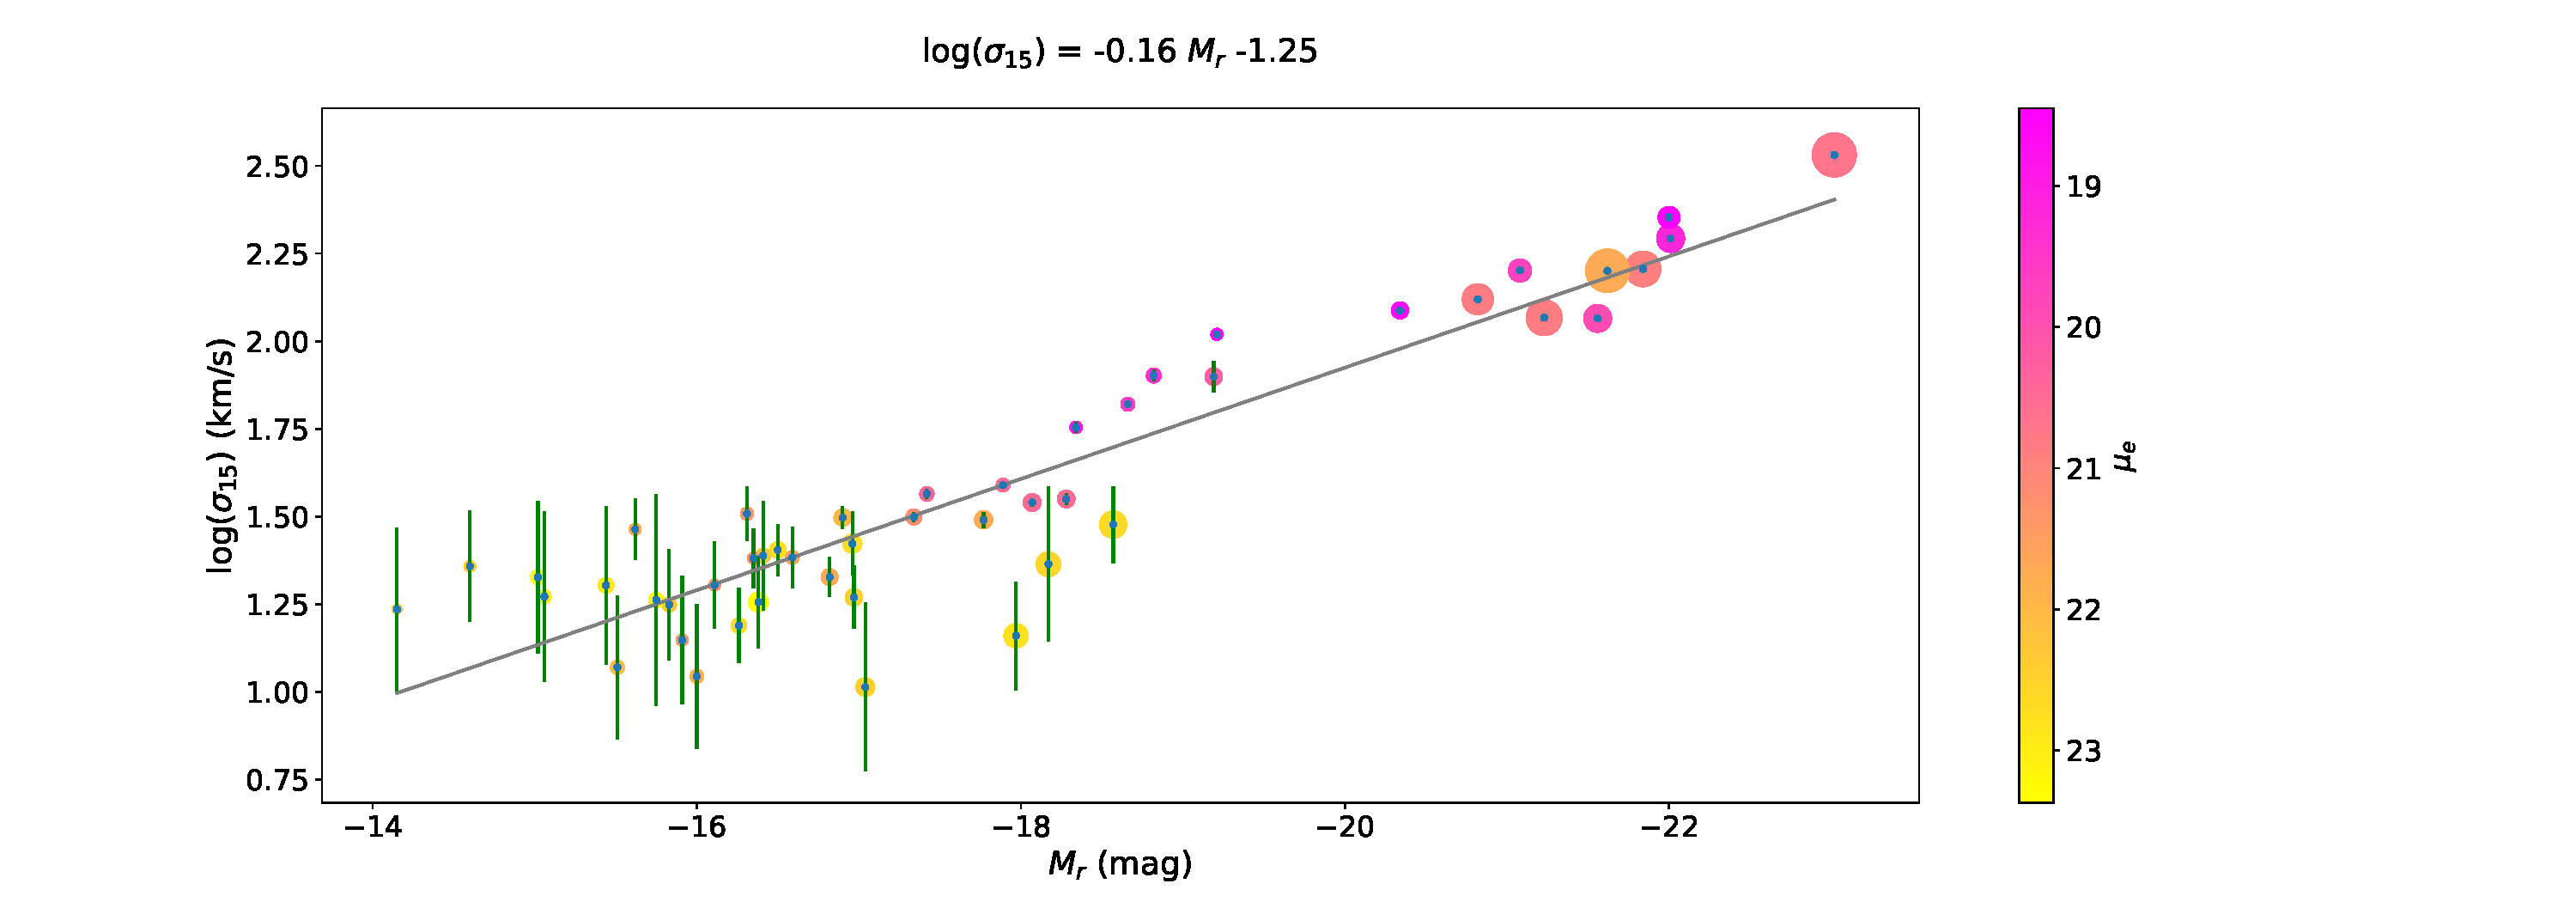
\includegraphics[width=20cm,height=8cm,keepaspectratio]
   {../2_pipeline/1_FJ/Faber_Jackson_x-axis=M_r_EXC.pdf}   
	\caption{Faber Jackson Relation - SAMI-Fornax galaxies color coded by surface brightness}
     \label{fig:FJ(SAMI)}
\end{figure*}

\begin{figure*}[!htb]
   \centering
   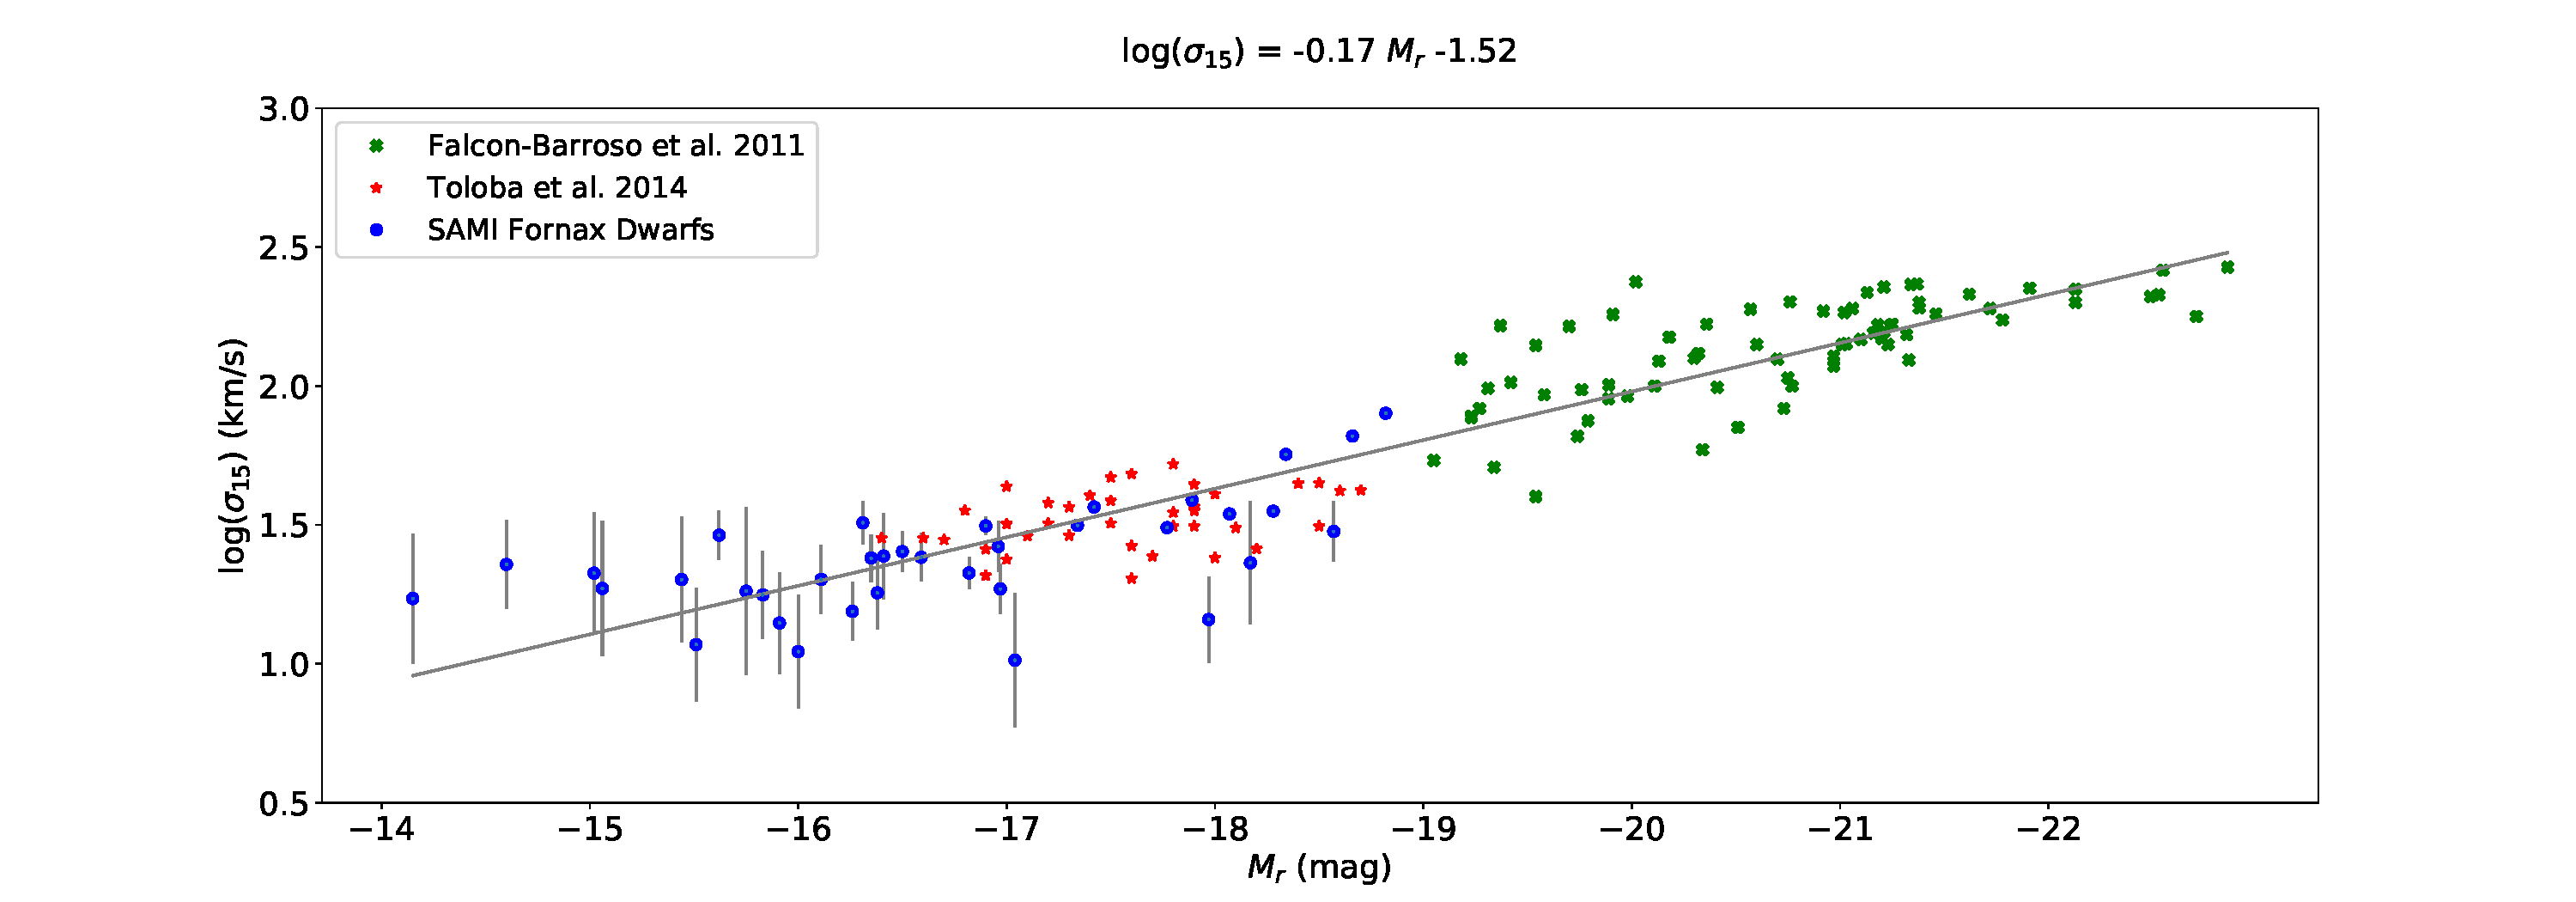
\includegraphics[width=17cm,height=9cm,keepaspectratio]
   {../2_pipeline/2_FJ_onlydE+useLiter/Faber_Jackson_onlyDWARF+useLiter.pdf}
	\caption{Faber Jackson Relation - SAMI-Fornax Dwarf ellipticals + Toloba et al. 2014 + Falcon-Barroso et al. 2010 }
     \label{fig:FJ(SAMI+Liter)}
\end{figure*}

One of the first discoveries in early-type galaxies was that their stellar velocity dispersion correlates with their luminosity (Faber \& Jackson 1967). This 2 dimensional realtion $L\propto\sigma^\alpha$, Faber-Jackson relation is in fact a projection
%a narrow plane called%
 of Fundamental Plane. 
% It has been shown that the slope of this relations gets shallower as it goes to fainter objects (Davies et al. 1983). 
In Fig.\ref{fig:FJ(SAMI)} we go down to faint low-mass galaxies of $M\sim 10^{7.4}M_\odot$, color coded by surface brightness within effective radius.
As we go to fainter objects we continue to have tight relation, only low-surface brightness galaxies ($\mu_r\approx 23$) as expected \textbf{[?]} are deviating from the line.  
The field-of-view of SAMI is small and in case of giants they cover only the central part. So from now on instead of using giant ellipticals of SAMI-Fornax we will use similar literature works such as Toloba et al. 2014 and Falcon-Barroso et al. 2011. \textbf{[a small explanation of Their work and data]}. The seen same slope in Fig.\ref{fig:FJ(SAMI)} slope from giants to dwarf ellipticals indicates their similar internal structure. The up-turn at the end of the tail might be a signature of dark matter in faint dwarf galaxies, but it also has to be kept in mind that this could be the limitation of data as we go down to faint object. As can be seen in Fig.\ref{fig:ObserRatio}, the ratio of successful observation to the initial target selection is quite small. So the galaxies at the end of the tail might be just tip of an iceberg.\\
In paper I angular-momentum of these objects was studied, where dwarf galaxies were not rotating significantly. The average perpendicular distance of our galaxies to the best fitted Faber Jackson line (Fig. 2), respect to different parameters such as $\lambda_R$, $<\mu_r>$, $g-r$, and $log(\sigma)$ are shown in Fig.4. As indicated above there is a clear relation between surface brightness and residuals. Moreover, \textbf{[??]} \textbf{[add three more plots for this section]}

%As central velocity dispersion is an indicator of total mass in dispersion supported galaxies, a complimentary comparison would be between stellar mass and velocity dispersion of these objects Fg.\ref{fig:M-S}. 

\section{Fundamental Plane}

\begin{figure*}[!htb]
   \centering
%   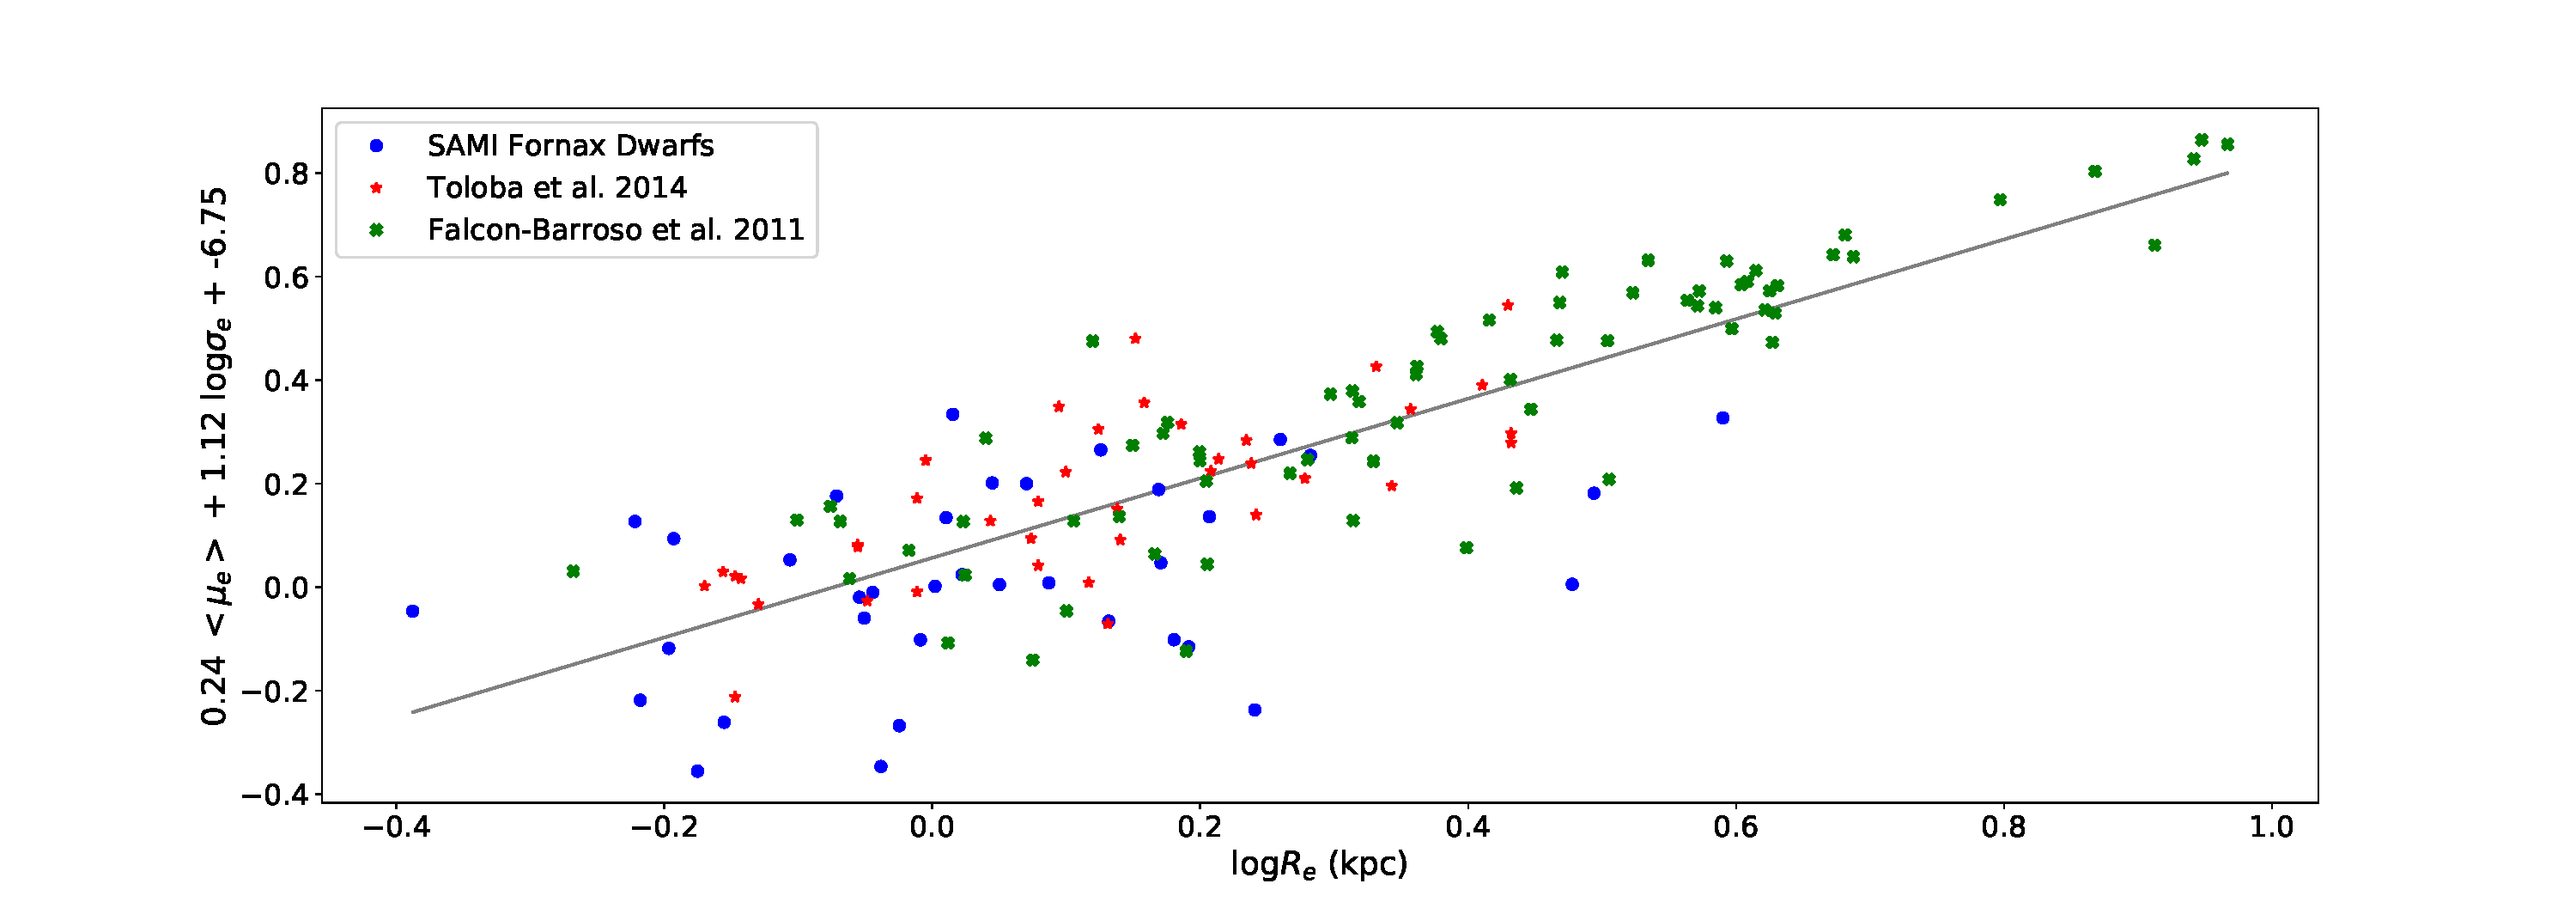
\includegraphics[width=20cm,height=8cm,keepaspectratio]{../2_pipeline/2_FP_LAD_onlydE+useLiter/FP_LAD+Liter_x=logR_DWARF.pdf}
  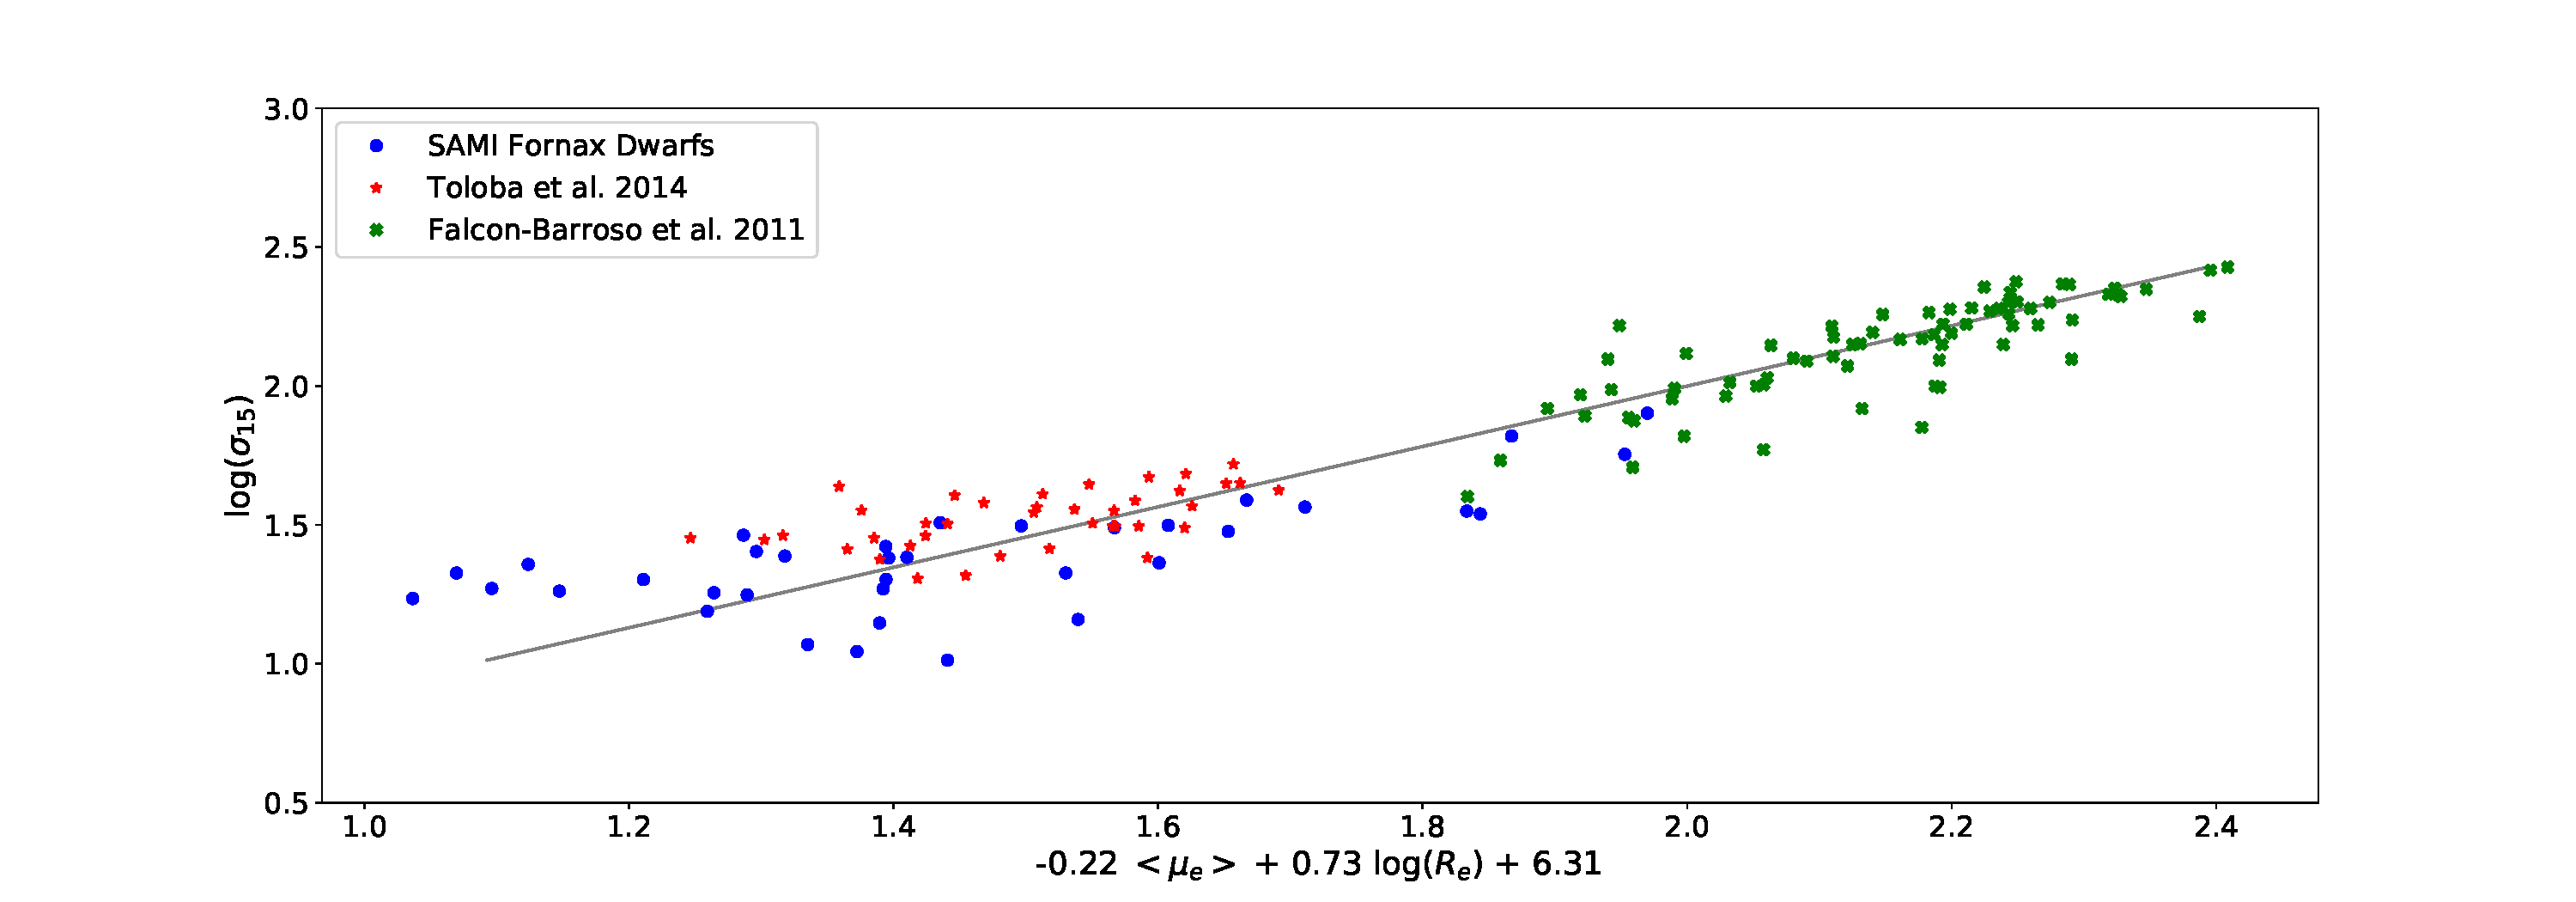
\includegraphics[width=20cm,height=8cm,keepaspectratio]{../2_pipeline/2_FP_LAD_onlydE+useLiter/rev_FP_LAD+Liter_x=logS_DWARF.pdf}
         \caption{Fundamental plane in two different Projections}
         \label{fig:FP}
\end{figure*}

The empirical Fundamental plane which is a bivariate relation (Brosche 1973, Dressler et al. 1973 and Djorgovski \& Davis 1987) between $R_e$ (the half light ration radius of the galaxy), $I_e$ (the mean surface brightness within Re in flux units), and $\sigma$ (the galaxy internal velocity dispersion), is an indication of galaxies being in virial equilibrium $R_e \propto \sigma^2 I_e^{-1} (M/L)^{-1}$ (Binney \& Tremaine 2008). By assuming the mass-to-light ratio M/L to be a power-law function of $\sigma$ and $I_e$, the physical quantities can be replaced by observables and the edge-on view of FP will be simplified to
\begin{eqnarray}
	log(R_e) = \alpha log(\sigma) + \beta <\mu_e> + \gamma
\end{eqnarray}
where $<\mu_e>$ is the mean surface brightness in $mag/arcsec^{2}$ defined as $-2.5log(I_e)+cte$. 
In this 3D space, elliptical galaxies lie on the plane with small scatter of $\sim0.1$ dex (Jorgensen et al. 1996; Bernardi et al. 2003), but other dynamically hot systems follow the planes with significantly different slopes and intercept values (Burstein et al. 1997; Schaeffer et al. 1993). Also the derived coefficients of FP (Bernardi et al 2003) are not exactly the same as the predicted ones from the virial theorem. This deviation of coefficients (tilt) also tightness of the plane have always been some of the keys for better understanding the evolution of galaxies, their structure and stellar population, or even dark matter distribution within different galaxies (Renzini \& Ciotti 1993; Borriello et al. 2003).
%The observed coefficients of FP are different from the predicted ones of the virial theorem. This 'tilt' of the FP might be due to different formation histories and evolutionary processes, or it can be explained by the evolution of M/L as a function of stellar population (age, metalicity, and initial mass function), also possible dark matter content.
In the edge-on view of FP (eq. 1) all distance-dependent quantities, velocity dispersion and surface brightness, are collected in one side. The inverse relation between $R_e$ and $I_e$ is one of the keys to existence of the FP, which in the face-on view $log(\sigma) = \alpha' log(R_e) + \beta' <\mu_e> + \gamma'$ they are in one side. For calculation of error bars in this projection we use covariance matrix between $R_e$ and $\mu_e$ of FDS, table. ??.

There are multiple ways to define the residuals to the plane and find this best fitted plane in the three dimensional space of ($logR_e$, $\mu_e$, $log\sigma$). In the direct method (Bernardi et al. 2003) residuals along one axis (mostly $r_e$) is minimized, while in the orthogonal fit the three-dimensional orthogonal fit is minimized. The most common way for the FP, also our chosen method, is the least absolute deviation instead of the usual least-square deviation (e.g. J\o rgensen et al. 1996, Falc$\acute{o}$n-Barroso et la. 2011, and Cappellari et al. 2013) as it's relatively insensitive to few outliers and more robust by treating all parameters symmetrically (Jorgensen et al. 1996; La Barbera et al. 2010). Also in comparison with other results of various studies, it's important that the same method was used throughout all works. So the residuals perpendicular to the plane are 
\begin{eqnarray}
	D = \frac{| log(R_e)-\alpha log(\sigma)-\beta <\mu_e>-\gamma |}{\sqrt{\alpha^2+\beta^2+1}}
\end{eqnarray}
Even though the FP in Fig.\ref{fig:FP} is derived from least-absolute deviation method, the FP we got from least-square deviation was quite similar since we do not have any significant outliers in SAMI-Fornax data.
The uncertainties of coefficients are derived by bootstrap procedure \textbf{[To Do]}.

The best orthogonal fits for our SAMI-Fornax sample, Toloba et al. 2014, and Faber-Jackson 2011 are\\
\textit{face-on view}:
\begin{eqnarray}
    log(\sigma) = 0.73\;log(R_e) - 0.22 <\mu_e> +\;6.30
\end{eqnarray}
\textit{edge-on view}:
\begin{eqnarray}
	log(R_e) = 1.12\;log(\sigma) + 0.24 <\mu_e> -\;6.75
\end{eqnarray}

As expected since one more parameter is included in the fitting of FP compared to FJ, the scatters of points become less. In contrast to previous works (e.g. Kourkchi et al. 2012, Toloba et al. 2012), we see that faint dwarf galaxies lie on the FP of their brighter counterpart. And again the upturn of dEs in the faintest region might be due to selection effect, since the S/N of galaxies with lower dispersions could be too low to measure kinematics on.
\\The rms scatter about the FP is ?? dex. \textbf{[To Do]}

%In integrated galaxy specra, lines broadening  can be caused by both velocity dispersion and the galaxy's rotational velocity. The effect of $V_{rot}$ will more prominent in elongated rotational galaxies such as FCC177 and FCC153. Without considering their rotational velocity they will deviate from FP, so we didn't include them in FP fitting.

%Zartisky et al. 2006 argues that a simple plane is not enough to explain this unifying relationship. 

%... But since our galaxy is concentrated on elliptical galaxies and so dispersion supported $\sigma$ is the measure of the mass of each galaxy...\cite{Barat2019}

%... Replacing velocity dispersions of our giant galaxies with Fornax3D results did not show prominent difference in FP. So we will stick with SAMI-fornax results for both giant and dwarf galaxies, as standard properties calculated from different methods are tended to have different systematic errors. ... 

I conclude this section by placing ....
... suggesting a physical connection ...


\subsection{Fundamental Plane in $\kappa$-space}
\begin{figure}[!htb]
   \centering
   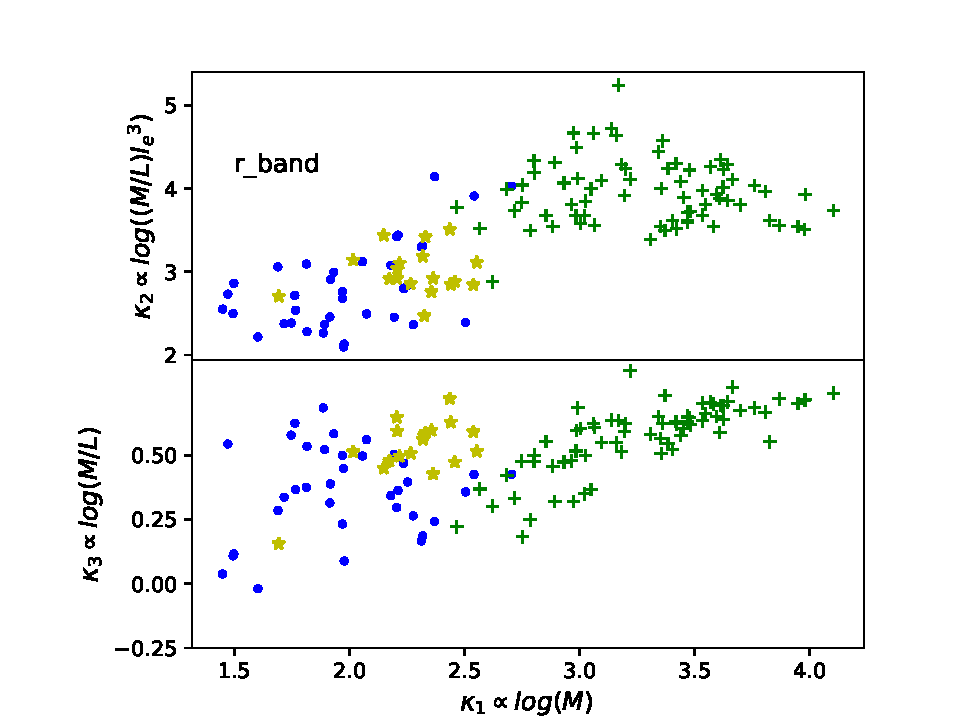
\includegraphics[width=10cm,height=8cm,keepaspectratio]
   {../2_pipeline/2_FP_kappa+Liter/FP_kappa+Liter_DWARF.pdf}
         \caption{FP in $\kappa$ space}
         \label{fig:FPkappa}
\end{figure}

We conclude this section by studying the FP in $\kappa$-space (Bender et al. 1992).
For more transparent analysis of FP a new coordinate system is introduced, by a simple orthogonal coordinate transformation of the 3 dimensional space of ($logR_e$, $logI_e$, $log\sigma^2$). By defining luminosity and mass as $L=c_1\,I_e\,{r_e}^2$ and $M=c_2\,{\sigma_0}^2\,r_2$, each of the coordinates will have a specific physical meaning. $\kappa_1$ being representative of galaxies size or logarithm of mass, $\kappa_2$ being representative of the logarithm of $M/L$ and $\kappa_3$ is proportional to the logarithm of $(M/L)\;{\mu_e}^3$. Also in $\kappa$ coordinate system $\kappa_1-\kappa_2$ and $\kappa_1-\kappa_3$ projections correspond to face-on and edge-on viwe of FP respectively.\\
In Fig.\ref{fig:FPkappa} the projections of SAMI-Fornax galaxies and recent similar studies in $kappa$-space are illustrated. Their observations were done in V and K band, so by using transformations between magnitude systems we transform them to r band first. The different behavior of giant and dwarf ellipticals in the $\kappa_1-\kappa_2$ space is an indication of their different formation scenarios.  \textbf{[what else we see?]}
%when we have a young and a faint galaxy, the younger galaxy has lower $\mu$ and so is brighter compared to the old galaxy. Also the color of the older one is redder. This fact is called fading.%

\section{Color vs. $\sigma$}
To see also the relation of dynamical mass of the galaxies with their stellar population w can use $\sigma$-color diagram. In Fig.\ref{fig:CI-S} we see almost a linear trend between various central colors and velocity dispersion of the whole sample of dEs, except dwarfs which bend toward bluer regions. The scatter around this relation can e due to the difference in age, metallicity and also star formation history of galaxies. 

\begin{figure*}[!htb]
   \centering
   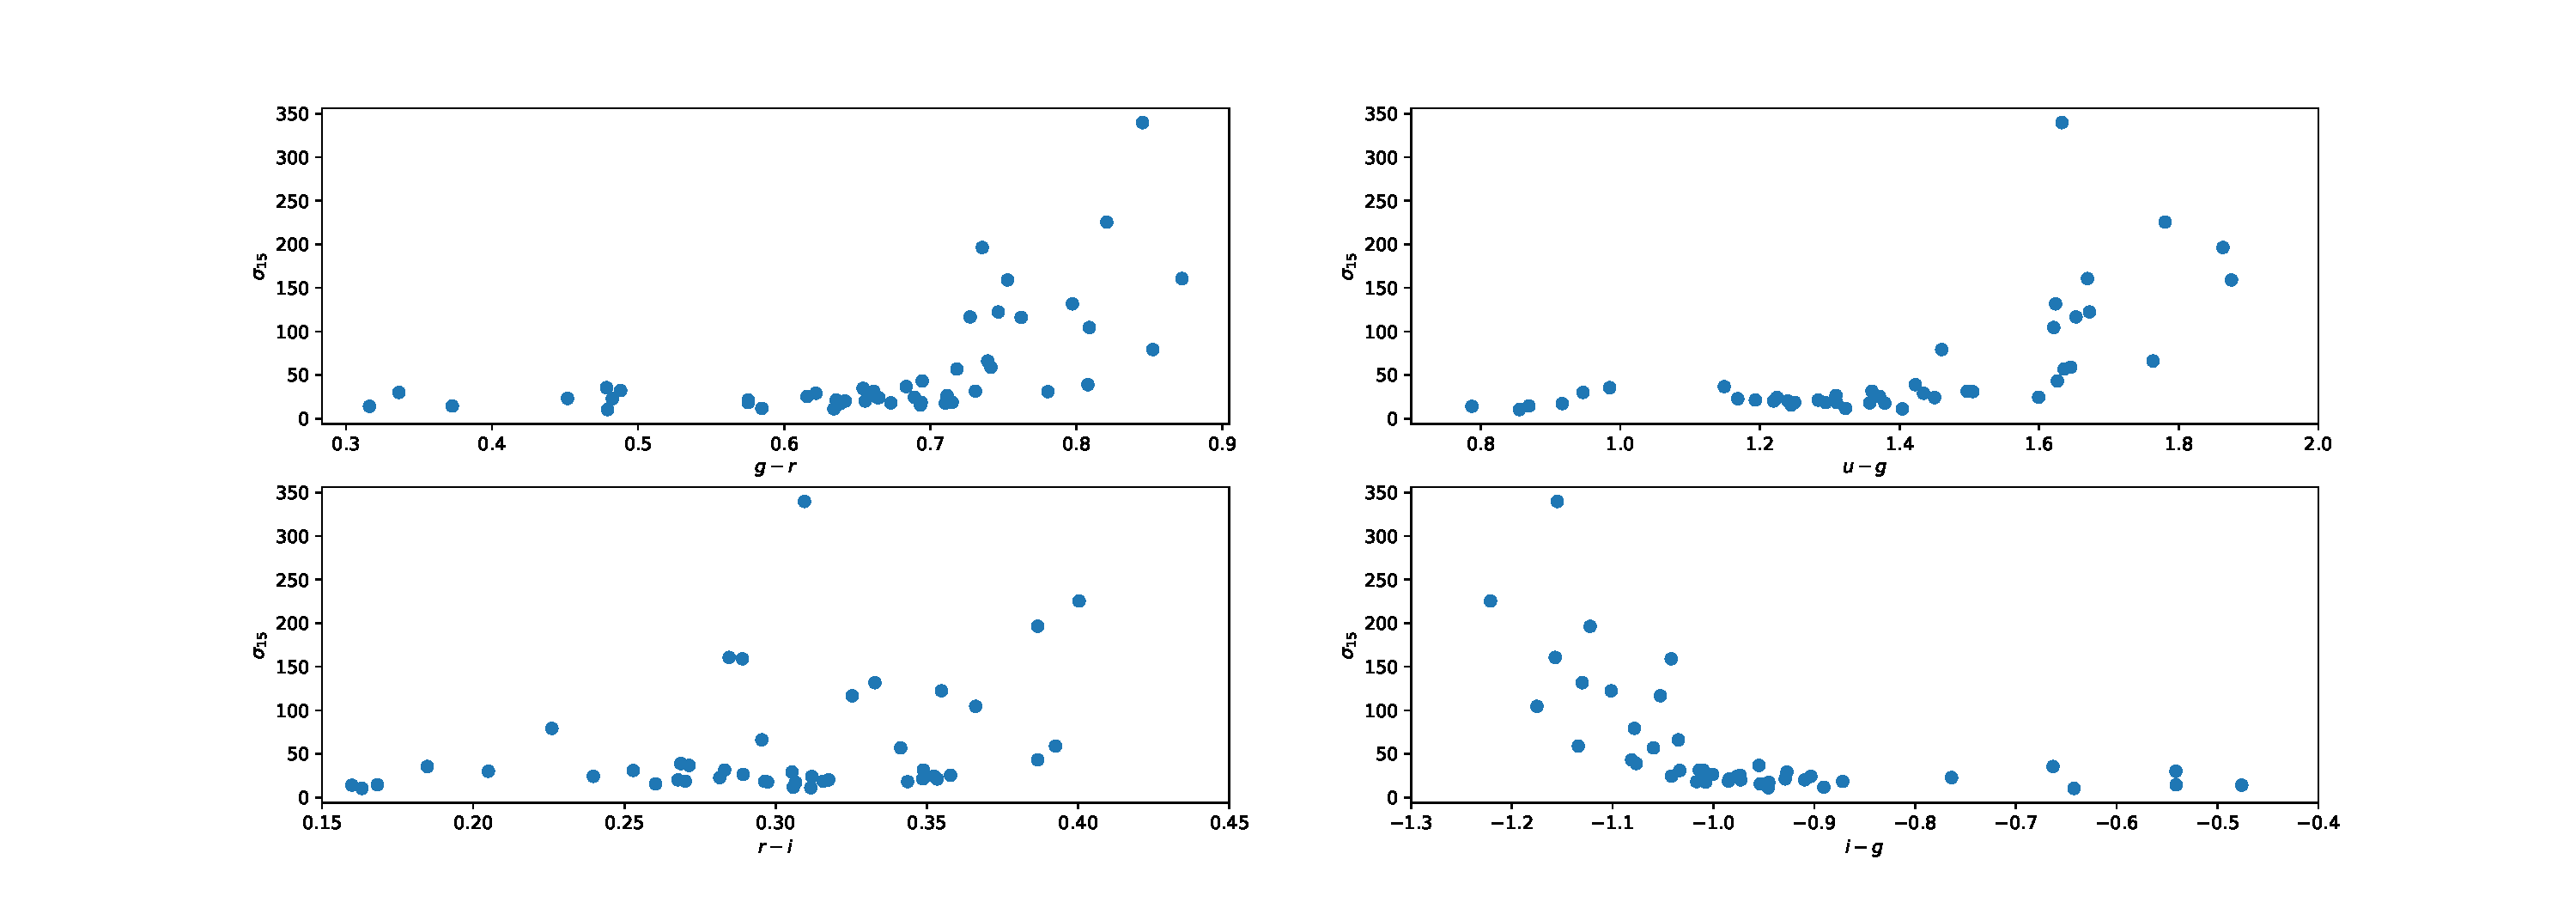
\includegraphics[width=20cm,height=20cm,keepaspectratio]{../2_pipeline/1_color_Disp/Color_Disp.pdf}
         \caption{Color vs. Dispersion}
         \label{fig:CI-S}
\end{figure*}


\begin{table*}
\begin{center}
\caption{}
{\renewcommand{\arraystretch}{1.}
\resizebox{18cm}{!} {
\begin{tabular}{|cccccc|}
\hline 
FCC & log($M_*/M_{\odot})_r$ & $\sigma$(km/s) & log($L_{r,1/2}$($L_{Sun}$) & log($M_{dyn,1/2}$)($M_{Sun}$) & $(M/L)_r$($M_{Sun}/L_{Sun}$) \\
\hline \hline
213 & 11.28$\pm$0.0020 & 339.81$\pm$6.48 & 10.76$\pm$0.032 & 12.07$\pm$0.016 & 20.33$\pm$1.68 \\
167 & 10.89$\pm$0.0019 & 143.40$\pm$1.21 & 10.35$\pm$0.024 & 10.91$\pm$0.007 & 3.55$\pm$0.20 \\
219 & 10.96$\pm$0.0018 & 154.30$\pm$3.28 & 10.35$\pm$0.020 & 10.74$\pm$0.018 & 2.44$\pm$0.15 \\
184 & 10.81$\pm$0.0021 & 143.40$\pm$1.70 & 10.29$\pm$0.036 & 11.12$\pm$0.010 & 6.87$\pm$0.59 \\
276 & 10.65$\pm$0.0025 & 123.30$\pm$0.64 & 10.20$\pm$0.044 & 11.17$\pm$0.004 & 9.37$\pm$0.95 \\
29 & 10.69$\pm$0.0020 & 116.12$\pm$1.01 & 10.18$\pm$0.0280 & 10.72$\pm$0.007 & 3.47$\pm$0.2321 \\
179 & 10.5091$\pm$0.0024 & 70.0000$\pm$1.4730 & 10.0470$\pm$0.0400 & 10.5115$\pm$0.0183 & 2.9145$\pm$0.2951 \\
147 & 10.4283$\pm$0.0020 & 131.1000$\pm$1.4951 & 9.9870$\pm$0.0240 & 10.6537$\pm$0.0099 & 4.6418$\pm$0.2775 \\
83 & 10.4017$\pm$0.0023 & 102.8000$\pm$0.5972 & 9.8830$\pm$0.0400 & 10.7156$\pm$0.0051 & 6.8017$\pm$0.6315 \\
193 & 10.1979$\pm$0.0020 & 95.3000$\pm$1.3667 & 9.6910$\pm$0.0200 & 10.0978$\pm$0.0125 & 2.5520$\pm$0.1385 \\
249 & 9.8011$\pm$0.0020 & 103.8000$\pm$0.5797 & 9.2390$\pm$0.0200 & 9.8340$\pm$0.0049 & 3.9355$\pm$0.1865 \\
190 & 9.6728$\pm$0.0022 & 74.6200$\pm$7.8886 & 9.2310$\pm$0.0280 & 9.9045$\pm$0.0918 & 4.7157$\pm$1.0424 \\ \hline
277 & 9.4690$\pm$0.0022 & 80.1700$\pm$2.9007 & 9.0830$\pm$0.0280 & 9.8149$\pm$0.0314 & 5.3947$\pm$0.5229 \\
143 & 9.4560$\pm$0.0022 & 62.3100$\pm$1.0189 & 9.0190$\pm$0.0240 & 9.5293$\pm$0.0142 & 3.2382$\pm$0.2079 \\
235 & 9.0386$\pm$0.0034 & 29.9744$\pm$7.4942 & 8.9830$\pm$0.0560 & 9.5283$\pm$0.2172 & 3.5104$\pm$1.8128 \\
301 & 9.3652$\pm$0.0022 & 48.7400$\pm$1.8700 & 8.8910$\pm$0.0240 & 9.2051$\pm$0.0333 & 2.0611$\pm$0.1949 \\
263 & 9.0004$\pm$0.0027 & 28.0000$\pm$1.3586 & 8.8670$\pm$0.0360 & 9.0595$\pm$0.0421 & 1.5579$\pm$0.1988 \\
37 & 9.0192$\pm$0.0033 & 23.1160$\pm$11.7317 & 8.8230$\pm$0.0560 & 9.2064$\pm$0.4408 & 2.4178$\pm$2.4738 \\
33 & 9.2439$\pm$0.0027 & 34.6622$\pm$0.9357 & 8.7830$\pm$0.0400 & 9.2558$\pm$0.0235 & 2.9707$\pm$0.3172 \\
285 & 8.7834$\pm$0.0035 & 14.4437$\pm$5.1387 & 8.7430$\pm$0.0600 & 8.7817$\pm$0.3090 & 1.0933$\pm$0.7925 \\
182 & 9.1682$\pm$0.0024 & 39.2000$\pm$0.4939 & 8.7110$\pm$0.0320 & 9.1205$\pm$0.0109 & 2.5675$\pm$0.1999 \\
136 & 9.0824$\pm$0.0028 & 30.9298$\pm$1.5543 & 8.6630$\pm$0.0440 & 9.1723$\pm$0.0437 & 3.2308$\pm$0.4611 \\
106 & 8.8965$\pm$0.0027 & 36.6946$\pm$1.2047 & 8.5230$\pm$0.0360 & 9.1050$\pm$0.0285 & 3.8201$\pm$0.4040 \\
202 & 8.9093$\pm$0.0028 & 31.5052$\pm$1.0090 & 8.4910$\pm$0.0440 & 9.0684$\pm$0.0278 & 3.7799$\pm$0.4531 \\
113 & 8.4790$\pm$0.0035 & 10.3114$\pm$5.6974 & 8.3710$\pm$0.0560 & 8.2520$\pm$0.4799 & 0.7605$\pm$0.8461 \\
222 & 8.7708$\pm$0.0033 & 18.6047$\pm$3.8464 & 8.3430$\pm$0.0520 & 8.6946$\pm$0.1796 & 2.2469$\pm$0.9672 \\
100 & 8.7505$\pm$0.0035 & 26.4483$\pm$5.5318 & 8.3390$\pm$0.0560 & 9.0893$\pm$0.1817 & 5.6275$\pm$2.4634 \\
203 & 8.7570$\pm$0.0033 & 31.3815$\pm$2.3254 & 8.3150$\pm$0.0520 & 9.1470$\pm$0.0644 & 6.7931$\pm$1.2943 \\
135 & 8.7083$\pm$0.0032 & 21.2401$\pm$2.7843 & 8.2830$\pm$0.0520 & 8.7707$\pm$0.1139 & 3.0742$\pm$0.8861 \\
207 & 8.5125$\pm$0.0030 & 24.1795$\pm$4.8484 & 8.1910$\pm$0.0440 & 8.6972$\pm$0.1742 & 3.2080$\pm$1.3269 \\
245 & 8.5729$\pm$0.0035 & 25.3773$\pm$4.3179 & 8.1550$\pm$0.0560 & 8.9193$\pm$0.1478 & 5.8126$\pm$2.1153 \\
252 & 8.5849$\pm$0.0032 & 24.4416$\pm$8.7130 & 8.1190$\pm$0.0480 & 8.7712$\pm$0.3096 & 4.4903$\pm$3.2396 \\
300 & 8.5498$\pm$0.0041 & 18.0232$\pm$5.4663 & 8.1070$\pm$0.0680 & 8.7786$\pm$0.2634 & 4.6953$\pm$2.9414 \\
266 & 8.4988$\pm$0.0028 & 24.0355$\pm$4.7049 & 8.0950$\pm$0.0360 & 8.5497$\pm$0.1700 & 2.8491$\pm$1.1401 \\
46 & 8.3101$\pm$0.0031 & 32.2014$\pm$5.6714 & 8.0790$\pm$0.0440 & 8.8942$\pm$0.1530 & 6.5342$\pm$2.3950 \\
188 & 8.4255$\pm$0.0035 & 15.4514$\pm$3.7701 & 8.0590$\pm$0.0520 & 8.4128$\pm$0.2119 & 2.2585$\pm$1.1348 \\
211 & 8.3387$\pm$0.0029 & 20.1410$\pm$5.7160 & 7.9990$\pm$0.0400 & 8.3749$\pm$0.2465 & 2.3763$\pm$1.3664 \\
164 & 8.3351$\pm$0.0034 & 11.0678$\pm$5.2301 & 7.9550$\pm$0.0520 & 8.0344$\pm$0.4105 & 1.2008$\pm$1.1439 \\
306 & 7.9136$\pm$0.0033 & 14.0366$\pm$5.9076 & 7.9190$\pm$0.0440 & 8.1039$\pm$0.3656 & 1.5310$\pm$1.2980 \\
253 & 8.3048$\pm$0.0036 & 17.7121$\pm$6.4887 & 7.8870$\pm$0.0560 & 8.4832$\pm$0.3182 & 3.9471$\pm$2.9364 \\
274 & 8.1779$\pm$0.0039 & 18.2740$\pm$12.6537 & 7.8550$\pm$0.0600 & 8.5531$\pm$0.6014 & 4.9908$\pm$6.9460 \\
298 & 8.1686$\pm$0.0033 & 29.0552$\pm$5.8133 & 7.8030$\pm$0.0440 & 8.7182$\pm$0.1738 & 8.2262$\pm$3.3956 \\
264 & 8.0985$\pm$0.0038 & 11.7375$\pm$5.5398 & 7.7590$\pm$0.0560 & 8.0992$\pm$0.4100 & 2.1890$\pm$2.0855 \\
195 & 8.1332$\pm$0.0041 & 20.1151$\pm$10.4218 & 7.7310$\pm$0.0640 & 8.6621$\pm$0.4500 & 8.5328$\pm$8.9308 \\
250 & 7.9732$\pm$0.0040 & 18.6780$\pm$10.4047 & 7.5790$\pm$0.0600 & 8.4559$\pm$0.4839 & 7.5320$\pm$8.4557 \\
178 & 7.9490$\pm$0.0043 & 21.2195$\pm$10.6095 & 7.5630$\pm$0.0680 & 8.6535$\pm$0.4343 & 12.3176$\pm$12.4674 \\
134 & 7.6366$\pm$0.0040 & 22.8041$\pm$8.3158 & 7.3950$\pm$0.0560 & 8.4788$\pm$0.3167 & 12.1280$\pm$8.9825 \\
51 & 7.5933$\pm$0.0037 & 17.1884$\pm$9.2307 & 7.2150$\pm$0.0520 & 8.0673$\pm$0.4665 & 7.1178$\pm$7.6923 \\ \hline
\end{tabular}
}}
\end{center}
\end{table*}

\section{Dynamical Mass}

Variety in dark matter fraction of dEs can be accounted as one of the reasons for deviation of dEs from FP (e.g. Reda et al. 2005) or even FP tilt (e.g. Cappellari et al. 2006, and Graves \& Faber 2010). We measure dynamical mass and dark matter fraction of our galaxies within SAMI field-of-view following Wolf et al. 2010. \\Not considering the difference between radial and tangential velocity dispersion weakens the accuracy of conclusions about structure and formation of galaxies. This becomes more important when calculating dynamical mass of a galaxy by only having its 2d observed radial properties. Wolf et al. 2010 using the spherical Jeans equation showed within $r_3$ radius this difference is insignificant. $r_3$ is where the log-slope of the 3D tracer density profile is -3, and for dispersion supported galaxies it is close to the 3D half-light radius $r_{1/2}$. So the dynamical mass will be defined as:
\begin{eqnarray}
	M_{1/2}\simeq930(\frac{{\sigma_{los}}^2}{{km}^2s^{-2}})(\frac{R_e}{pc})M_{\odot}
\end{eqnarray}
where $R_e$ is the 2D projected half-light radius and $\sigma_{los}$ is the line-of-sight velocity dispersion. In Fig.\ref{fig:ML} we expand the relationship between $M_{1/2}$ and the half-light luminosity $L_{1/2}=0.5L$ for elliptical and dwarf elliptical galaxies in different environments. The first thing we see is that our galaxies connect well with the brighter dwarfs of Toloba et al (2014) and elliptical galaxies of Falcon-Barroso et al. 2010 both within Virgo cluster also the Local Group dwarfs from Wolf et al (2010). This means that the dark matter properties of these dwarfs in clusters are the same as in the Local Group, implying that the dark matter distribution inside the galaxies is not affected by the cluster environment. The upturns of log(M/L) at both low and high $\sigma$s have been investigated before (e.g. Benson et al 2000; Marinonin \& Hudson 2002; van de Bosch et al. 2003; Zaritsky et al. 2006) and point to the two different galaxy formation history in the smallest and largest dark matter haloes. Winds and UV photonization are considered as the two main processes responsible for the increase of M/L with decreasing $\sigma$ in left side of the parabola by lowering star formation efficiency in low-mass systems. Supernovae winds remove material in the galaxies, and it's more prominent in low mass galaxies because of their weak potential well (Martin 1999; Dekel \& Woo 2003), while the intergalactic UV radiation is ionizing the gas (Babul \&Rees 1992).\\
Moreover, as emphasized in Wolf et al 2010 and Zaritsky et al. 2006 dEs are sitting at the minimum of the parabola relation between dynamical half-light mass-to-light ratio and velocity dispersion. Position of the minimum and its corresponding mass scales are important as it's the turnover point between two different star formation scenarios of bright and faint systems. Three different power-law regimes / two different regimes? what they mean? 

\begin{figure}[!htb]
   \centering
   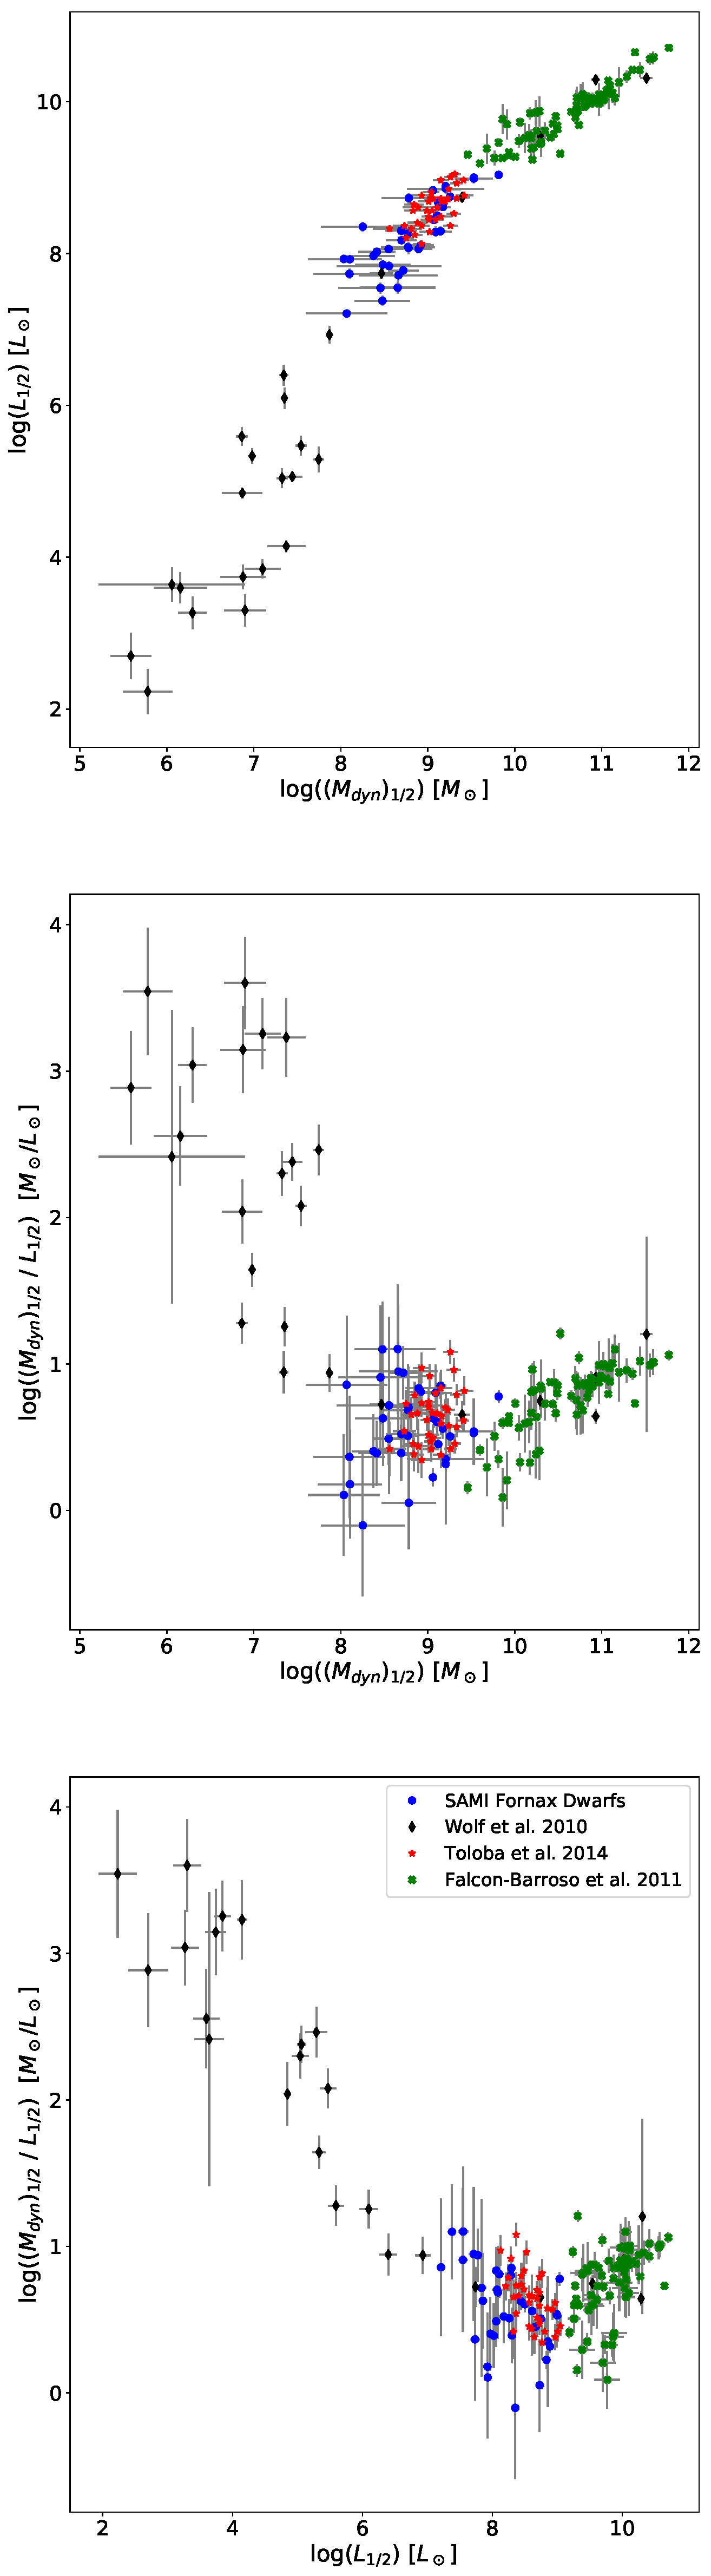
\includegraphics[height=25cm]{../2_pipeline/2_MassDyn_Luminosity+Liter/DyM-L+Liter_DWARF.pdf}   		
  	 \caption{Dynamical Mass vs. Luminosity ratio \textbf{[info box must be added]}}
         \label{fig:ML}
\end{figure}

\begin{figure}[!htb]
   \centering
   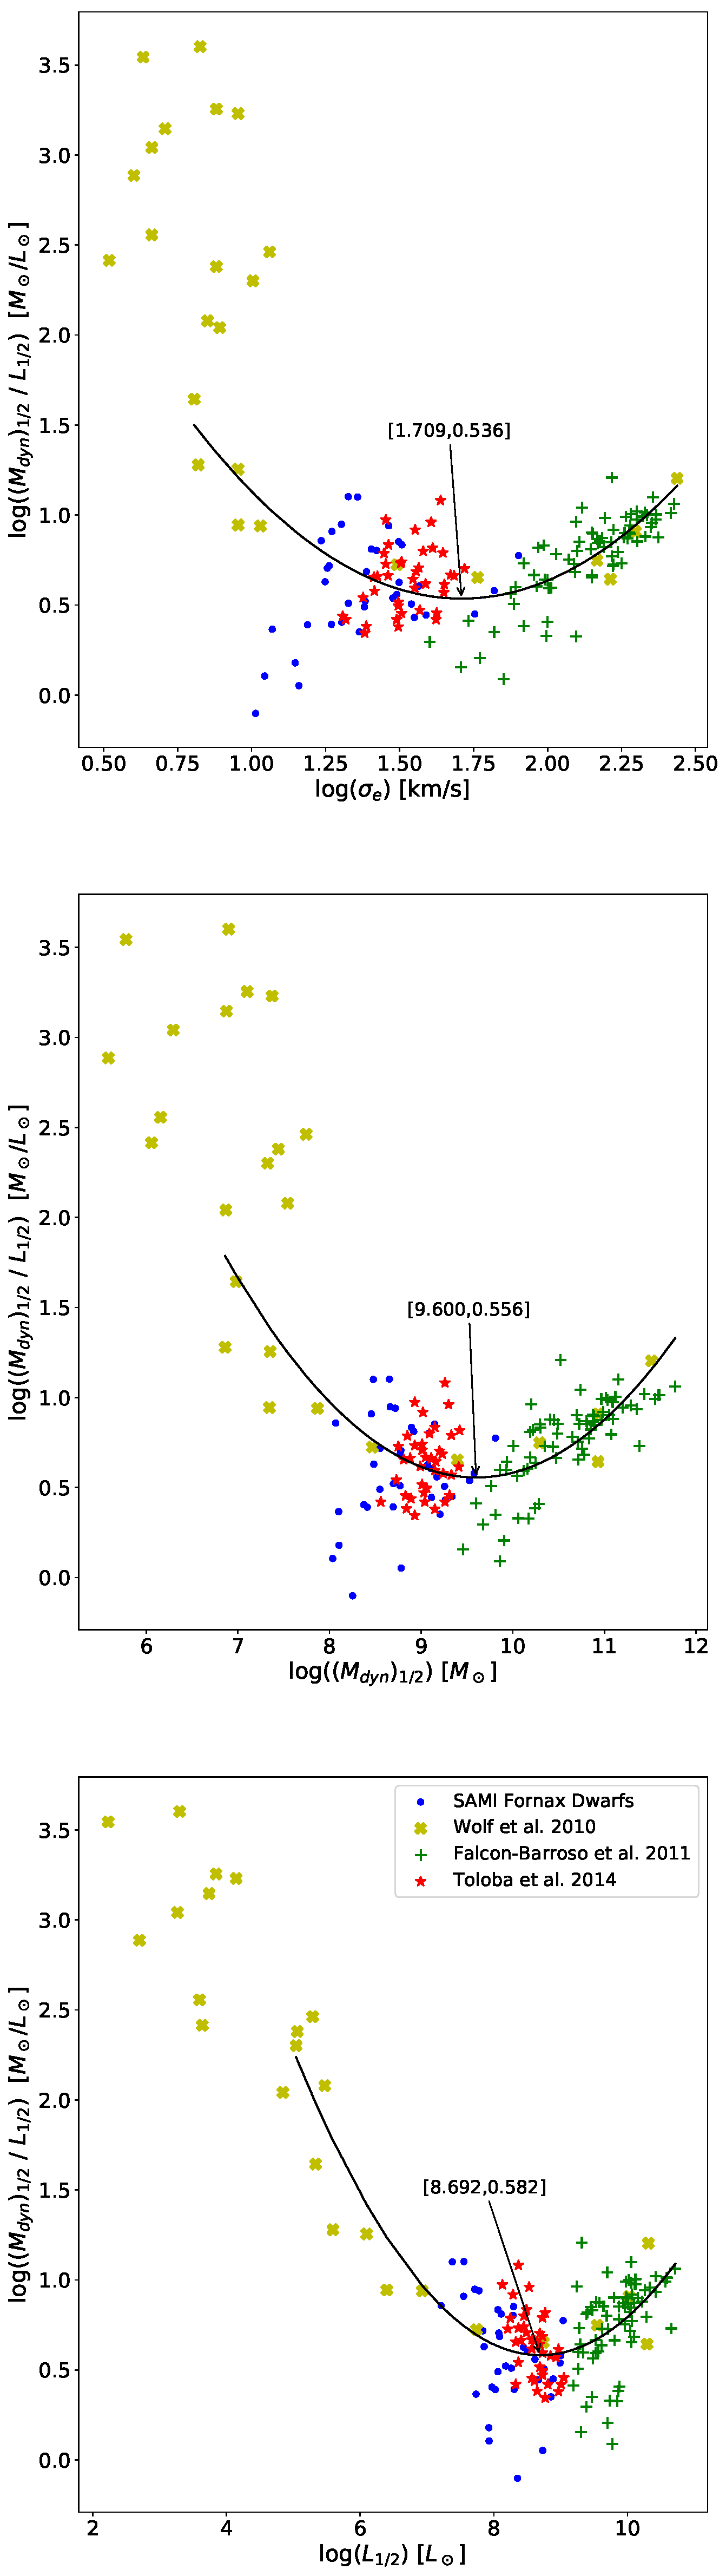
\includegraphics[height=25cm]{../2_pipeline/3_ParabolaFit_MassDyn/Paraola_DyM_DWARF.pdf}   		
  	 \caption{Dynamical Mass vs. Luminosity ratio \textbf{[info box must be added]}}
         \label{fig:ML}
\end{figure}

\subsection{Stellar Mass vs. / Sigma}

\begin{figure}[!htb]
   \centering
   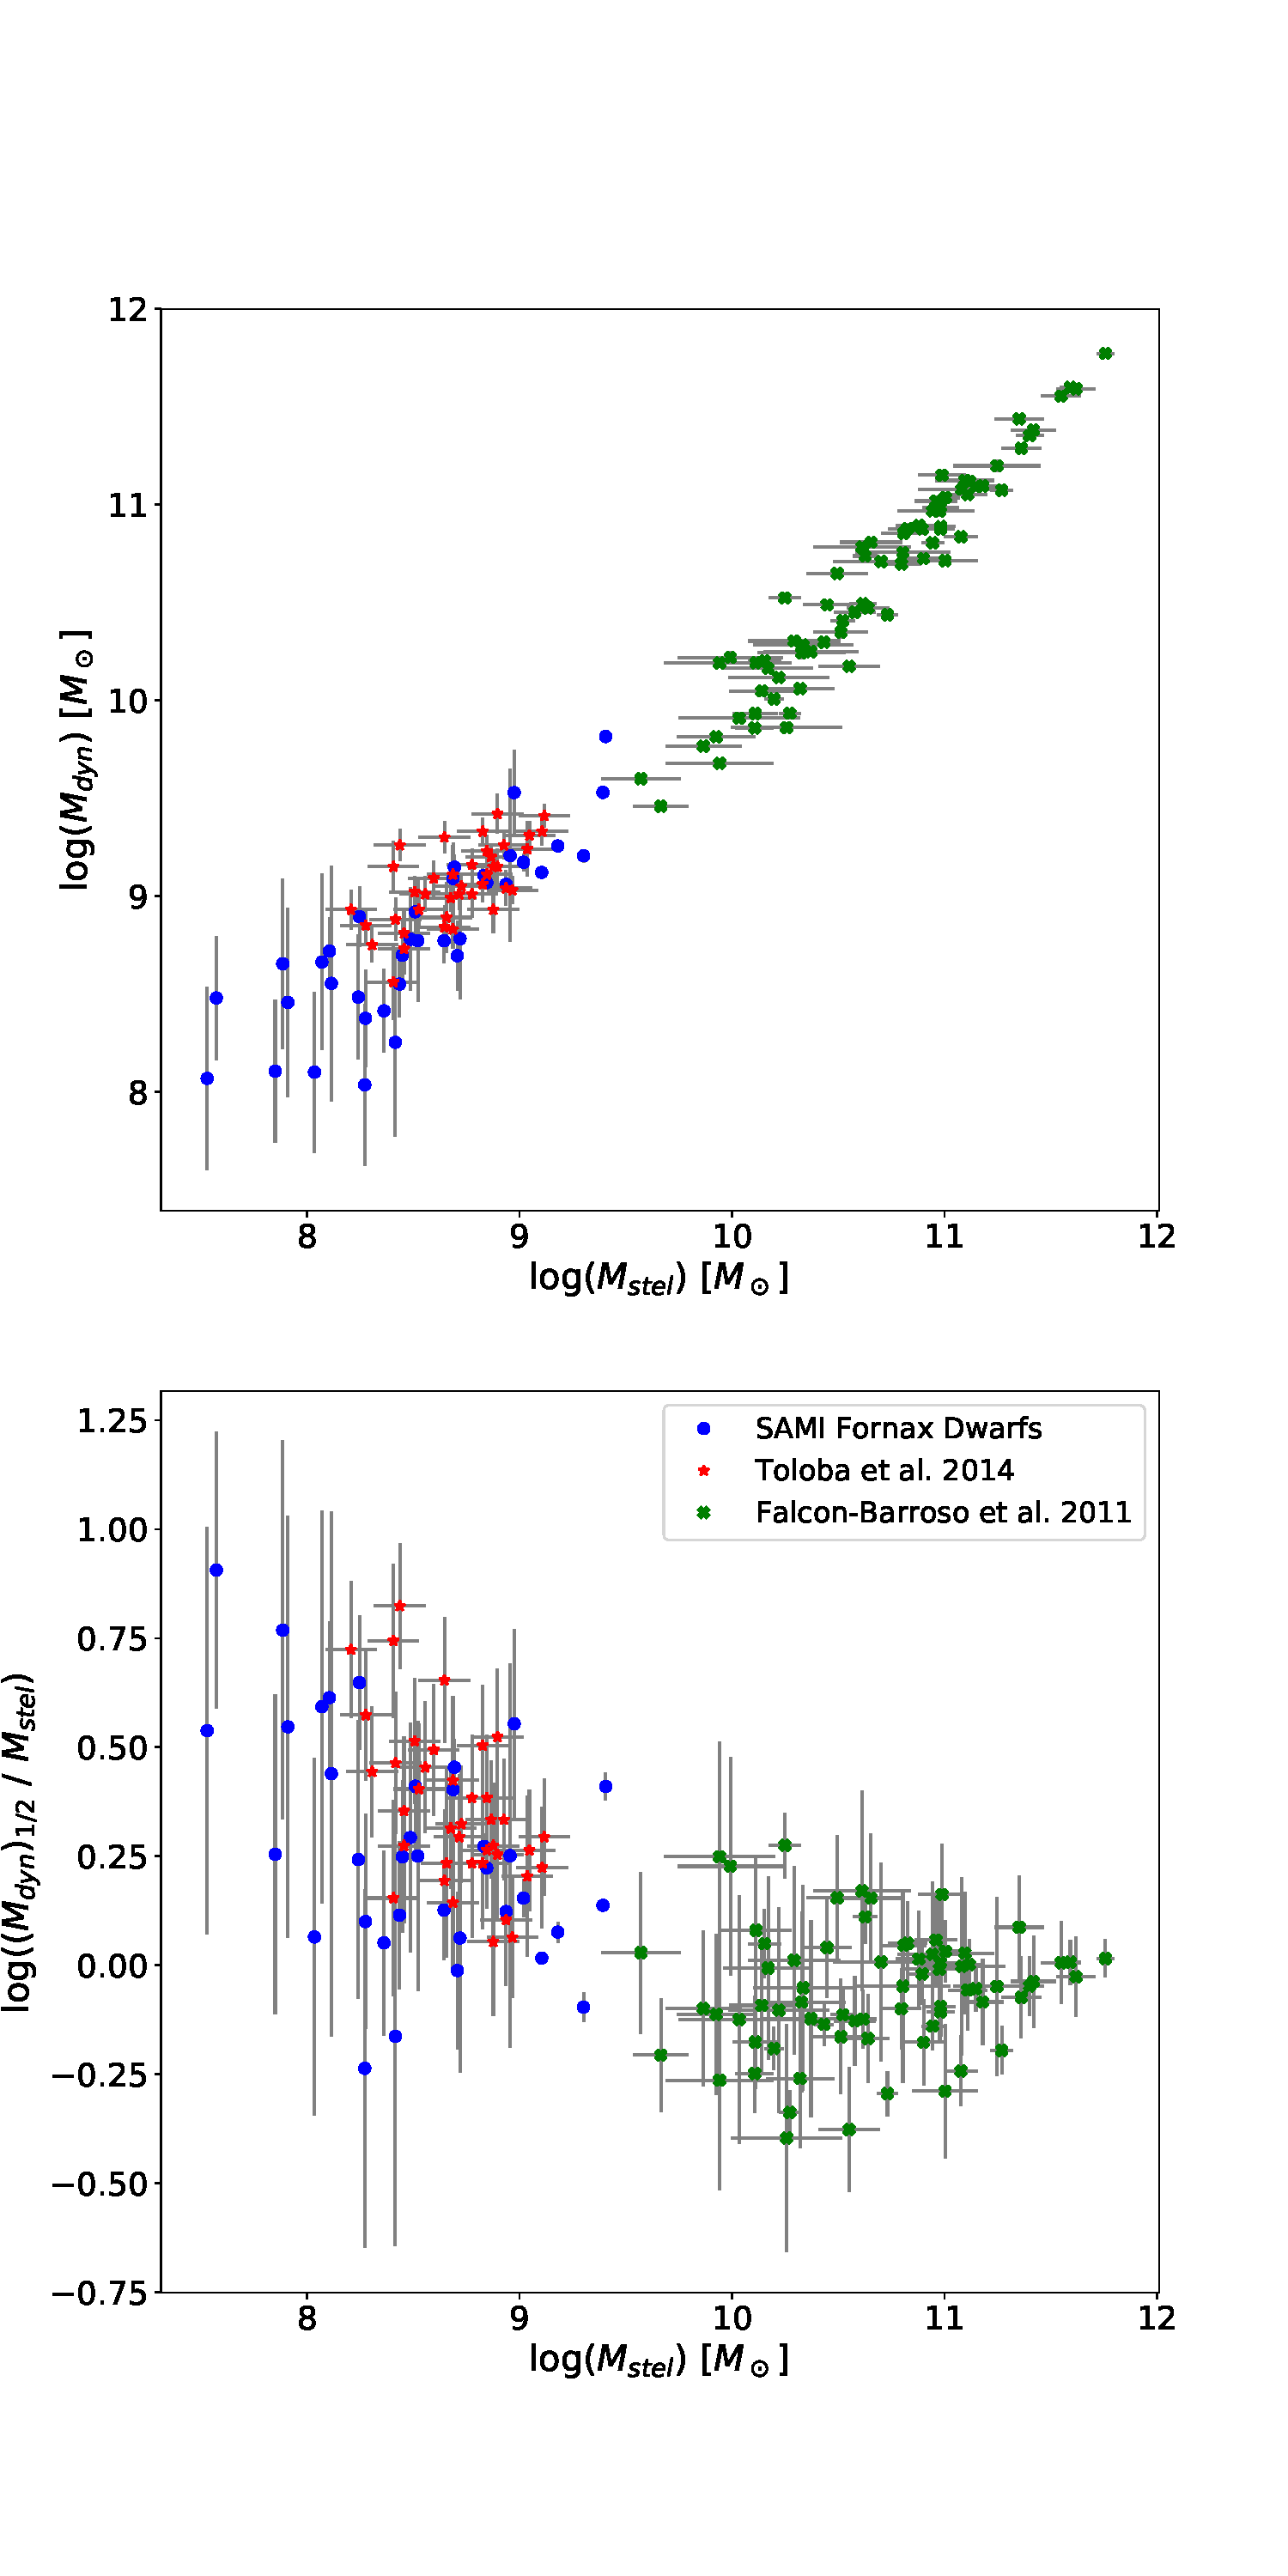
\includegraphics[width=8cm]{../2_pipeline/2_MassDyn_Luminosity+Liter/DyM_StM+Liter_DWARF.pdf}   		
  	 \caption{Stellar Mass vs. Luminosity ratio \textbf{[info box must be added]}}
         \label{fig:MM}
\end{figure}


\section{Phase-Space Diagrams}





%______________________________________________________________

\section{Conclusions}

  
\begin{acknowledgements}

\end{acknowledgements}


%-------------------------------------------------------------------
%\bibliographystyle{aa}
%\bibliography{references}

\end{document}

%%%%%%%%%%%%%%%%%%%%%%%%%%%%%%%%%%%%%%%%%%%%%%%%%%%%%%%%%%%%%%
Examples for figures using graphicx
A guide "Using Imported Graphics in LaTeX2e"  (Keith Reckdahl)
is available on a lot of LaTeX public servers or ctan mirrors.
The file is : epslatex.pdf 
%%%%%%%%%%%%%%%%%%%%%%%%%%%%%%%%%%%%%%%%%%%%%%%%%%%%%%%%%%%%%%

%_____________________________________________________________
%                 A figure as large as the width of the column
%-------------------------------------------------------------
   \begin{figure}
   \centering
   \includegraphics[width=\hsize]{empty.eps}
      \caption{Vibrational stability equation of state
               $S_{\mathrm{vib}}(\lg e, \lg \rho)$.
               $>0$ means vibrational stability.
              }
         \label{FigVibStab}
   \end{figure}
%
%_____________________________________________________________
%                                    One column rotated figure
%-------------------------------------------------------------
   \begin{figure}
   \centering
   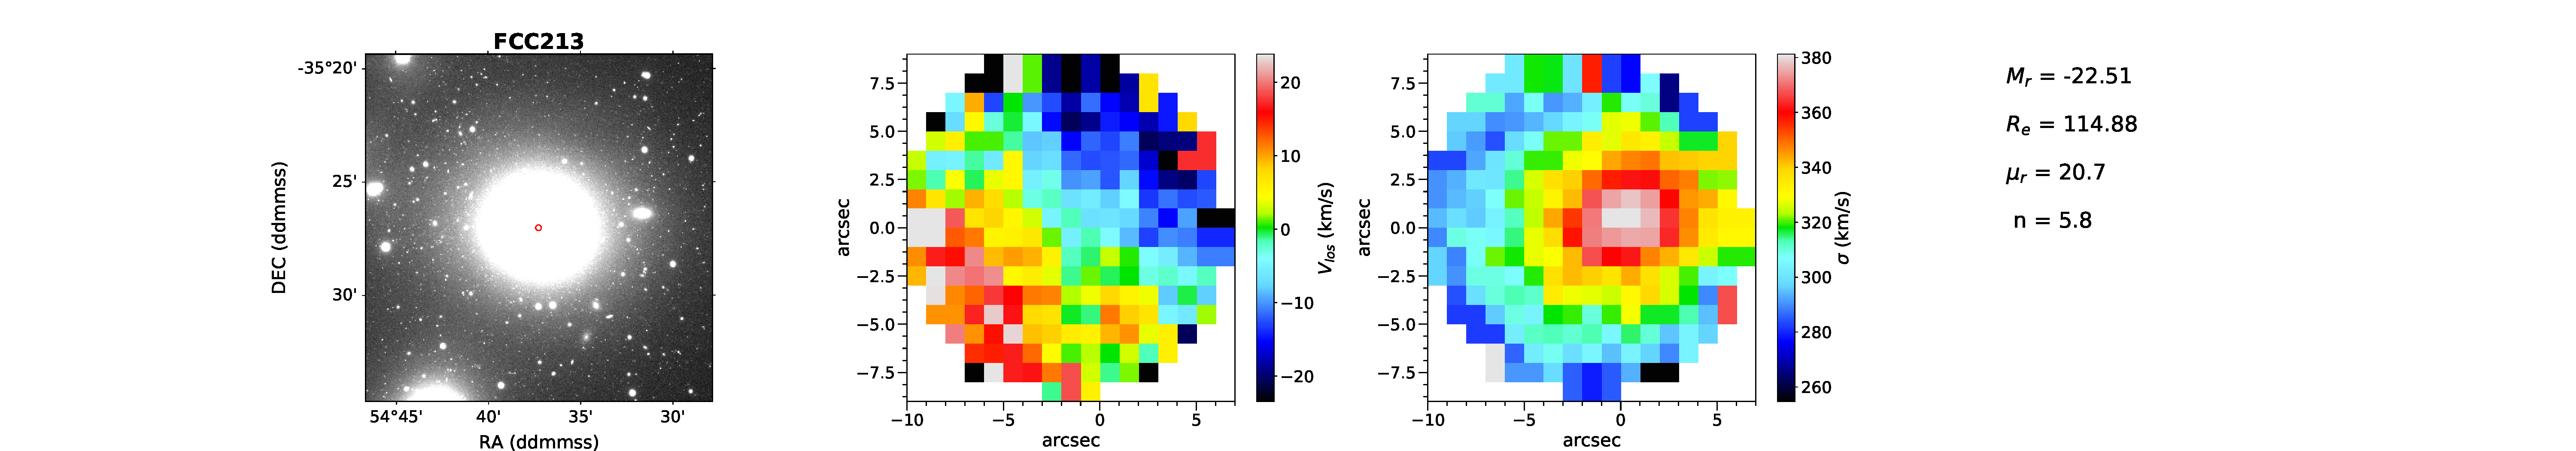
\includegraphics[angle=-90,width=3cm]{213Velocity_map.pdf}
      \caption{Vibrational stability equation of state
               $S_{\mathrm{vib}}(\lg e, \lg \rho)$.
               $>0$ means vibrational stability.
              }
         \label{FigVibStab}
   \end{figure}
%
%_____________________________________________________________
%                        Figure with caption on the right side 
%-------------------------------------------------------------
   \begin{figure}
   \sidecaption
   \includegraphics[width=3cm]{empty.eps}
      \caption{Vibrational stability equation of state
               $S_{\mathrm{vib}}(\lg e, \lg \rho)$.
               $>0$ means vibrational stability.
              }
         \label{FigVibStab}
   \end{figure}
%
%_____________________________________________________________
%
%_____________________________________________________________
%                                Figure with a new BoundingBox 
%-------------------------------------------------------------
   \begin{figure}
   \centering
   \includegraphics[bb=10 20 100 300,width=3cm,clip]{empty.eps}
      \caption{Vibrational stability equation of state
               $S_{\mathrm{vib}}(\lg e, \lg \rho)$.
               $>0$ means vibrational stability.
              }
         \label{FigVibStab}
   \end{figure}
%
%_____________________________________________________________
%
%_____________________________________________________________
%                                      The "resizebox" command 
%-------------------------------------------------------------
   \begin{figure}
   \resizebox{\hsize}{!}
            {\includegraphics[bb=10 20 100 300,clip]{empty.eps}
      \caption{Vibrational stability equation of state
               $S_{\mathrm{vib}}(\lg e, \lg \rho)$.
               $>0$ means vibrational stability.
              }}
         \label{FigVibStab}
   \end{figure}
%
%______________________________________________________________
%
%_____________________________________________________________
%                                             Two column Figure 
%-------------------------------------------------------------
   \begin{figure*}
   \resizebox{\hsize}{!}
           % {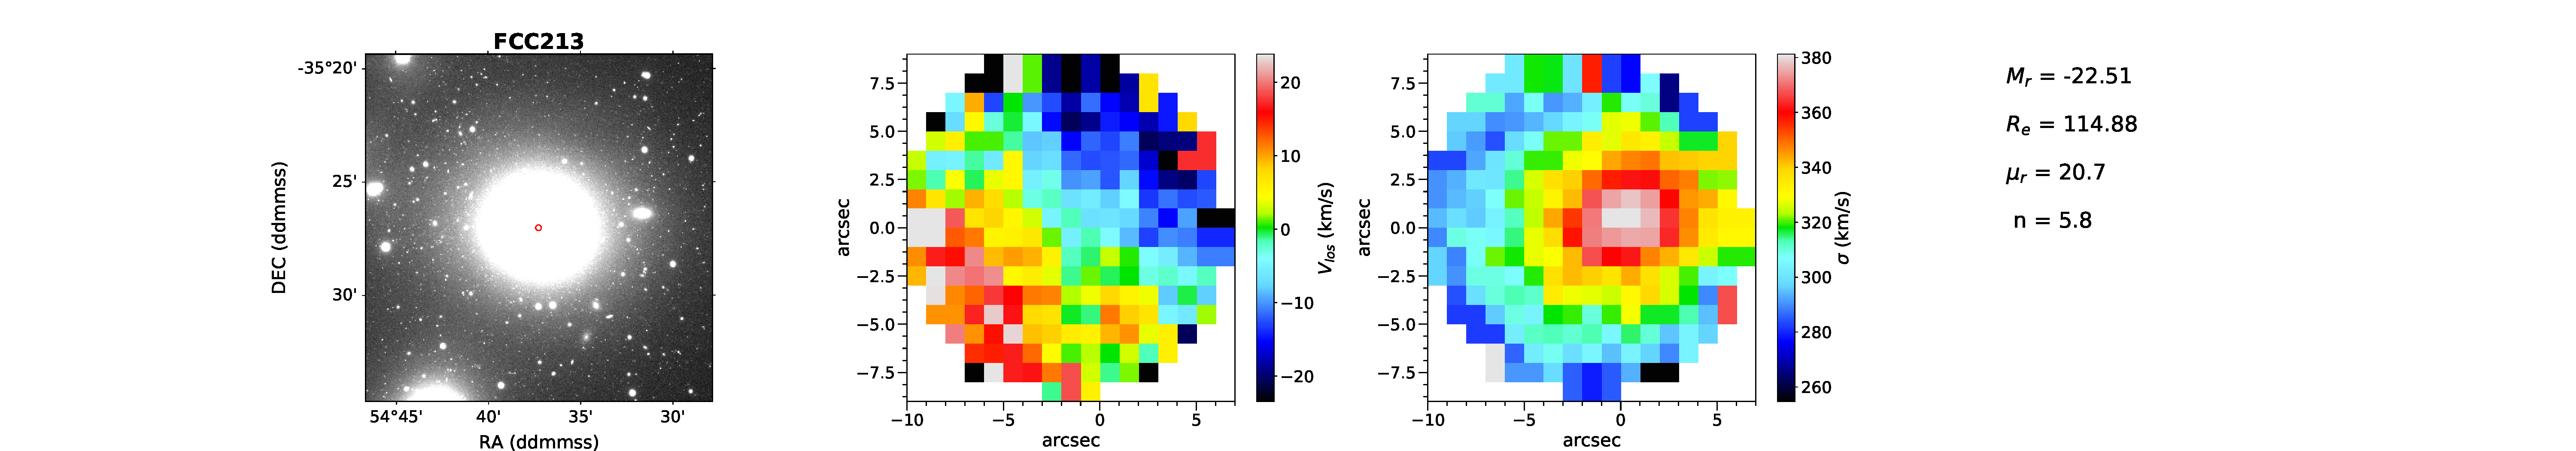
\includegraphics[bb=10 20 100 300,clip]{213Velocity_map.pdf}
      \caption{Vibrational stability equation of state
               $S_{\mathrm{vib}}(\lg e, \lg \rho)$.
               $>0$ means vibrational stability.
              }}
         \label{FigVibStab}
   \end{figure*}
%
%______________________________________________________________
%
%_____________________________________________________________
%                                             Simple A&A Table
%_____________________________________________________________
%
\begin{table}
\caption{Nonlinear Model Results}             % title of Table
\label{table:1}      % is used to refer this table in the text
\centering                          % used for centering table
\begin{tabular}{c c c c}        % centered columns (4 columns)
\hline\hline                 % inserts double horizontal lines
HJD & $E$ & Method\#2 & Method\#3 \\    % table heading 
\hline                        % inserts single horizontal line
   1 & 50 & $-837$ & 970 \\      % inserting body of the table
   2 & 47 & 877    & 230 \\
   3 & 31 & 25     & 415 \\
   4 & 35 & 144    & 2356 \\
   5 & 45 & 300    & 556 \\ 
\hline                                   %inserts single line
\end{tabular}
\end{table}
%
%_____________________________________________________________
%                                             Two column Table 
%_____________________________________________________________
%
\begin{table*}
\caption{Nonlinear Model Results}             
\label{table:1}      
\centering          
\begin{tabular}{c c c c l l l }     % 7 columns 
\hline\hline       
                      % To combine 4 columns into a single one 
HJD & $E$ & Method\#2 & \multicolumn{4}{c}{Method\#3}\\ 
\hline                    
   1 & 50 & $-837$ & 970 & 65 & 67 & 78\\  
   2 & 47 & 877    & 230 & 567& 55 & 78\\
   3 & 31 & 25     & 415 & 567& 55 & 78\\
   4 & 35 & 144    & 2356& 567& 55 & 78 \\
   5 & 45 & 300    & 556 & 567& 55 & 78\\
\hline                  
\end{tabular}
\end{table*}
%
%-------------------------------------------------------------
%                                          Table with notes 
%-------------------------------------------------------------
%
% A single note
\begin{table}
\caption{\label{t7}Spectral types and photometry for stars in the
  region.}
\centering
\begin{tabular}{lccc}
\hline\hline
Star&Spectral type&RA(J2000)&Dec(J2000)\\
\hline
69           &B1\,V     &09 15 54.046 & $-$50 00 26.67\\
49           &B0.7\,V   &*09 15 54.570& $-$50 00 03.90\\
LS~1267~(86) &O8\,V     &09 15 52.787&11.07\\
24.6         &7.58      &1.37 &0.20\\
\hline
LS~1262      &B0\,V     &09 15 05.17&11.17\\
MO 2-119     &B0.5\,V   &09 15 33.7 &11.74\\
LS~1269      &O8.5\,V   &09 15 56.60&10.85\\
\hline
\end{tabular}
\tablefoot{The top panel shows likely members of Pismis~11. The second
panel contains likely members of Alicante~5. The bottom panel
displays stars outside the clusters.}
\end{table}
%
% More notes
%
\begin{table}
\caption{\label{t7}Spectral types and photometry for stars in the
  region.}
\centering
\begin{tabular}{lccc}
\hline\hline
Star&Spectral type&RA(J2000)&Dec(J2000)\\
\hline
69           &B1\,V     &09 15 54.046 & $-$50 00 26.67\\
49           &B0.7\,V   &*09 15 54.570& $-$50 00 03.90\\
LS~1267~(86) &O8\,V     &09 15 52.787&11.07\tablefootmark{a}\\
24.6         &7.58\tablefootmark{1}&1.37\tablefootmark{a}   &0.20\tablefootmark{a}\\
\hline
LS~1262      &B0\,V     &09 15 05.17&11.17\tablefootmark{b}\\
MO 2-119     &B0.5\,V   &09 15 33.7 &11.74\tablefootmark{c}\\
LS~1269      &O8.5\,V   &09 15 56.60&10.85\tablefootmark{d}\\
\hline
\end{tabular}
\tablefoot{The top panel shows likely members of Pismis~11. The second
panel contains likely members of Alicante~5. The bottom panel
displays stars outside the clusters.\\
\tablefoottext{a}{Photometry for MF13, LS~1267 and HD~80077 from
Dupont et al.}
\tablefoottext{b}{Photometry for LS~1262, LS~1269 from
Durand et al.}
\tablefoottext{c}{Photometry for MO2-119 from
Mathieu et al.}
}
\end{table}
%
%-------------------------------------------------------------
%                                       Table with references 
%-------------------------------------------------------------
%
\begin{table*}[h]
 \caption[]{\label{nearbylistaa2}List of nearby SNe used in this work.}
\begin{tabular}{lccc}
 \hline \hline
  SN name &
  Epoch &
 Bands &
  References \\
 &
  (with respect to $B$ maximum) &
 &
 \\ \hline
1981B   & 0 & {\it UBV} & 1\\
1986G   &  $-$3, $-$1, 0, 1, 2 & {\it BV}  & 2\\
1989B   & $-$5, $-$1, 0, 3, 5 & {\it UBVRI}  & 3, 4\\
1990N   & 2, 7 & {\it UBVRI}  & 5\\
1991M   & 3 & {\it VRI}  & 6\\
\hline
\noalign{\smallskip}
\multicolumn{4}{c}{ SNe 91bg-like} \\
\noalign{\smallskip}
\hline
1991bg   & 1, 2 & {\it BVRI}  & 7\\
1999by   & $-$5, $-$4, $-$3, 3, 4, 5 & {\it UBVRI}  & 8\\
\hline
\noalign{\smallskip}
\multicolumn{4}{c}{ SNe 91T-like} \\
\noalign{\smallskip}
\hline
1991T   & $-$3, 0 & {\it UBVRI}  &  9, 10\\
2000cx  & $-$3, $-$2, 0, 1, 5 & {\it UBVRI}  & 11\\ %
\hline
\end{tabular}
\tablebib{(1)~\citet{branch83};
(2) \citet{phillips87}; (3) \citet{barbon90}; (4) \citet{wells94};
(5) \citet{mazzali93}; (6) \citet{gomez98}; (7) \citet{kirshner93};
(8) \citet{patat96}; (9) \citet{salvo01}; (10) \citet{branch03};
(11) \citet{jha99}.
}
\end{table*}
%_____________________________________________________________
%                      A rotated Two column Table in landscape  
%-------------------------------------------------------------
\begin{sidewaystable*}
\caption{Summary for ISOCAM sources with mid-IR excess 
(YSO candidates).}\label{YSOtable}
\centering
\begin{tabular}{crrlcl} 
\hline\hline             
ISO-L1551 & $F_{6.7}$~[mJy] & $\alpha_{6.7-14.3}$ 
& YSO type$^{d}$ & Status & Comments\\
\hline
  \multicolumn{6}{c}{\it New YSO candidates}\\ % To combine 6 columns into a single one
\hline
  1 & 1.56 $\pm$ 0.47 & --    & Class II$^{c}$ & New & Mid\\
  2 & 0.79:           & 0.97: & Class II ?     & New & \\
  3 & 4.95 $\pm$ 0.68 & 3.18  & Class II / III & New & \\
  5 & 1.44 $\pm$ 0.33 & 1.88  & Class II       & New & \\
\hline
  \multicolumn{6}{c}{\it Previously known YSOs} \\
\hline
  61 & 0.89 $\pm$ 0.58 & 1.77 & Class I & \object{HH 30} & Circumstellar disk\\
  96 & 38.34 $\pm$ 0.71 & 37.5& Class II& MHO 5          & Spectral type\\
\hline
\end{tabular}
\end{sidewaystable*}
%_____________________________________________________________
%                      A rotated One column Table in landscape  
%-------------------------------------------------------------
\begin{sidewaystable}
\caption{Summary for ISOCAM sources with mid-IR excess 
(YSO candidates).}\label{YSOtable}
\centering
\begin{tabular}{crrlcl} 
\hline\hline             
ISO-L1551 & $F_{6.7}$~[mJy] & $\alpha_{6.7-14.3}$ 
& YSO type$^{d}$ & Status & Comments\\
\hline
  \multicolumn{6}{c}{\it New YSO candidates}\\ % To combine 6 columns into a single one
\hline
  1 & 1.56 $\pm$ 0.47 & --    & Class II$^{c}$ & New & Mid\\
  2 & 0.79:           & 0.97: & Class II ?     & New & \\
  3 & 4.95 $\pm$ 0.68 & 3.18  & Class II / III & New & \\
  5 & 1.44 $\pm$ 0.33 & 1.88  & Class II       & New & \\
\hline
  \multicolumn{6}{c}{\it Previously known YSOs} \\
\hline
  61 & 0.89 $\pm$ 0.58 & 1.77 & Class I & \object{HH 30} & Circumstellar disk\\
  96 & 38.34 $\pm$ 0.71 & 37.5& Class II& MHO 5          & Spectral type\\
\hline
\end{tabular}
\end{sidewaystable}
%
%_____________________________________________________________
%                              Table longer than a single page  
%-------------------------------------------------------------
% All long tables will be placed automatically at the end, after 
%                                        \end{thebibliography}
%
\begin{longtab}
\begin{longtable}{lllrrr}
\caption{\label{kstars} Sample stars with absolute magnitude}\\
\hline\hline
Catalogue& $M_{V}$ & Spectral & Distance & Mode & Count Rate \\
\hline
\endfirsthead
\caption{continued.}\\
\hline\hline
Catalogue& $M_{V}$ & Spectral & Distance & Mode & Count Rate \\
\hline
\endhead
\hline
\endfoot
%%
Gl 33    & 6.37 & K2 V & 7.46 & S & 0.043170\\
Gl 66AB  & 6.26 & K2 V & 8.15 & S & 0.260478\\
Gl 68    & 5.87 & K1 V & 7.47 & P & 0.026610\\
         &      &      &      & H & 0.008686\\
Gl 86 
\footnote{Source not included in the HRI catalog. See Sect.~5.4.2 for details.}
         & 5.92 & K0 V & 10.91& S & 0.058230\\
\end{longtable}
\end{longtab}
%
%_____________________________________________________________
%                              Table longer than a single page
%                                             and in landscape 
%  In the preamble, use:       \usepackage{lscape}
%-------------------------------------------------------------
% All long tables will be placed automatically at the end, after
%                                        \end{thebibliography}
%
\begin{longtab}
\begin{landscape}
\begin{longtable}{lllrrr}
\caption{\label{kstars} Sample stars with absolute magnitude}\\
\hline\hline
Catalogue& $M_{V}$ & Spectral & Distance & Mode & Count Rate \\
\hline
\endfirsthead
\caption{continued.}\\
\hline\hline
Catalogue& $M_{V}$ & Spectral & Distance & Mode & Count Rate \\
\hline
\endhead
\hline
\endfoot
%%
Gl 33    & 6.37 & K2 V & 7.46 & S & 0.043170\\
Gl 66AB  & 6.26 & K2 V & 8.15 & S & 0.260478\\
Gl 68    & 5.87 & K1 V & 7.47 & P & 0.026610\\
         &      &      &      & H & 0.008686\\
Gl 86
\footnote{Source not included in the HRI catalog. See Sect.~5.4.2 for details.}
         & 5.92 & K0 V & 10.91& S & 0.058230\\
\end{longtable}
\end{landscape}
\end{longtab}
%
% Online Material
%_____________________________________________________________
%        Online appendices have to be placed at the end, after
%                                        \end{thebibliography}
%-------------------------------------------------------------
%\end{thebibliography}

\Online

\begin{appendix} %First online appendix
\section{Background galaxy number counts and shear noise-levels}
Because the optical images used in this analysis...

\begin{figure*}
\centering
\includegraphics[width=16.4cm,clip]{1787f24.ps}
\caption{Plotted above...}
\label{appfig}
\end{figure*}

Because the optical images...
\end{appendix}

\begin{appendix} %Second online appendix
These studies, however, have faced...
\end{appendix}

%\end{document}
%
%_____________________________________________________________
%        Some tables or figures are in the printed version and
%                      some are only in the electronic version
%-------------------------------------------------------------
%
% Leave all the tables or figures in the text, at their right place 
% and use the commands \onlfig{} and \onltab{}. These elements
% will be automatically placed at the end, in the section
% Online material.

\documentclass{aa}
...
\begin{document}
text of the paper...
\begin{figure*}%f1
\includegraphics[width=10.9cm]{1787f01.eps}
\caption{Shown in greyscale is a...}
\label{cl12301}
\end{figure*}
...
from the intrinsic ellipticity distribution.
% Figure 2 available electronically only
\onlfig{
\begin{figure*}%f2
\includegraphics[width=11.6cm]{1787f02.eps}
\caption {Shown in greyscale...}
\label{cl1018}
\end{figure*}
}

% Figure 3 available electronically only
\onlfig{
\begin{figure*}%f3
\includegraphics[width=11.2cm]{1787f03.eps}
\caption{Shown in panels...}
\label{cl1059}
\end{figure*}
}

\begin{figure*}%f4
\includegraphics[width=10.9cm]{1787f04.eps}
\caption{Shown in greyscale is...}
\label{cl1232}
\end{figure*}

\begin{table}%t1
\caption{Complexes characterisation.}\label{starbursts}
\centering
\begin{tabular}{lccc}
\hline \hline
Complex & $F_{60}$ & 8.6 &  No. of  \\
...
\hline
\end{tabular}
\end{table}
The second method produces...

% Figure 5 available electronically only
\onlfig{
\begin{figure*}%f5
\includegraphics[width=11.2cm]{1787f05.eps}
\caption{Shown in panels...}
\label{cl1238}
\end{figure*}
}

As can be seen, in general the deeper...
% Table 2 available electronically only
\onltab{
\begin{table*}%t2
\caption{List of the LMC stellar complexes...}\label{Properties}
\centering
\begin{tabular}{lccccccccc}
\hline  \hline
Stellar & RA & Dec & ...
...
\hline
\end{tabular}
\end{table*}
}

% Table 3 available electronically only
\onltab{
\begin{table*}%t3
\caption{List of the derived...}\label{IrasFluxes}
\centering
\begin{tabular}{lcccccccccc}
\hline \hline
Stellar & $f12$ & $L12$ &...
...
\hline
\end{tabular}
\end{table*}
}
\end{document}
%
%-------------------------------------------------------------
%     For the online material, table longer than a single page
%                 In the preamble for landscape case, use : 
%                                          \usepackage{lscape}
%-------------------------------------------------------------
\documentclass{aa}
\usepackage[varg]{txfonts}
\usepackage{graphicx}
\usepackage{lscape}

\begin{document}
text of the paper
% Table will be print automatically at the end, in the section Online material.
\onllongtab{
\begin{longtable}{lrcrrrrrrrrl}
\caption{Line data and abundances ...}\\
\hline
\hline
Def & mol & Ion & $\lambda$ & $\chi$ & $\log gf$ & N & e &  rad & $\delta$ & $\delta$ 
red & References \\
\hline
\endfirsthead
\caption{Continued.} \\
\hline
Def & mol & Ion & $\lambda$ & $\chi$ & $\log gf$ & B & C &  rad & $\delta$ & $\delta$ 
red & References \\
\hline
\endhead
\hline
\endfoot
\hline
\endlastfoot
A & CH & 1 &3638 & 0.002 & $-$2.551 &  &  &  & $-$150 & 150 &  Jorgensen et al. (1996) \\                    
\end{longtable}
}% End onllongtab

% Or for landscape, large table:

\onllongtab{
\begin{landscape}
\begin{longtable}{lrcrrrrrrrrl}
...
\end{longtable}
\end{landscape}
}% End onllongtab
\end{document}